\documentclass[usenames,dvipsnames]{beamer}
\usepackage{eulervm}
\usepackage{calligra}
\usepackage{mystyle1}
\usepackage{tikzsymbols}
\title[Entanglement using Knots]{\huge Entanglement Classification using Knots \\{\large PH3203 Term Project}}
\author[Seth, Das, Karmakar]{{ Sagnik Seth} {\tiny{22MS026}} \and { Jessica  Das}  {\tiny{22MS157}} \and { Sayan Karmakar}  {\tiny{22MS163}}}
\institute[]{Instructor: Prof. Sourin Das\\[0.2cm]
	\textit{Department of Physics, IISER Kolkata}}
\date{}
\usetheme{Madrid}
\definecolor{bubbles}{rgb}{0.91, 1.0, 1.0}
\usecolortheme{whale}
\setbeamercolor{normal text}{fg=black,bg=bubbles!70}
\setbeamercolor{structure}{fg=red, bg=violet}

\setbeamercolor{alerted text}{fg=red!85!black}

\setbeamercolor{item projected}{use=item,fg=black,bg=item.fg!35}
\beamertemplatenavigationsymbolsempty
\setbeamercolor*{palette primary}{use=structure,fg=structure.fg}
\setbeamercolor*{palette secondary}{use=structure,fg=structure.fg!95!black}
\setbeamercolor*{palette tertiary}{use=structure,fg=structure.fg!90!black}
\setbeamercolor*{palette quaternary}{use=structure,fg=structure.fg!95!black,bg=black!80}

\setbeamercolor*{framesubtitle}{fg=white}

\setbeamercolor*{block title}{parent=structure,bg=black!60}
\setbeamercolor*{block body}{fg=black,bg=black!10}
\setbeamercolor*{block title alerted}{parent=alerted text,bg=black!15}
\setbeamercolor*{block title example}{parent=example text,bg=black!15}





% \setbeamertemplate{footline}{
%     \hfill
%     \scriptsize{
%         \insertshortauthor \quad (\insertshorttitle) \quad \insertshortdate
%         \hspace{1cm}
%         \insertframenumber\,/\,\inserttotalframenumber
%     }
%     \hspace{0.5cm}
%     \vspace{0.2cm}
\titlegraphic{\includesvg[scale=0.3]{pics/Square_knot.svg}}
\begin{document}
	
	% \frame{\titlepage}
	\begin{frame}
		\tikz [remember picture,overlay]
    \node at
        ([yshift=1cm, xshift=-1cm]current page.south east) 
        %or: (current page.center)
        {\includesvg[scale=0.1]{pics/IISER-Kolkata-logo-vector-01.svg}};
		\titlepage
	\end{frame}
	
	
	\begin{frame}
		\begin{center}
			\textbf{\huge Basic Theoretical Background}
		\end{center}
	\end{frame}
	
	\begin{frame}{\textbf{\large Introduction to Quantum Information}}
		\begin{itemize}
			\item \onslide<2->{\textbf{Pure State }$\rightarrow$ described by a single vector in Hilbert space.}
			
			\item \onslide<3->{When a system is in a statistical ensemble of many pure states $\{\ket{\psi_i}\}$, with respective \textit{classical} probabilities $p_i$, such a state is called a \textbf{Mixed State}. We represent such states using the density operator: 
			\[
			\rho = \sum_i p_i \ket{\psi_i}\bra{\psi_i}
			\]
			where $p_i \geq 0$, $\sum\limits_i p_i = 1$, and $\ket{\psi_i}$ are pure states.}
			
			\item \onslide<4->{If one of the $p_i$ equals $1$, the state is a pure state, with the properties $\rho^2 = \rho$ and $\mathrm{Tr}(\rho^2) = 1$.}
			
			\item \onslide<5->{A quantum state $\rho_{AB}$ is \textbf{separable} if it can be written as:
			\[
			\rho_{AB} = \sum\limits_i p_i\, \rho_A^{(i)} \otimes \rho_B^{(i)}
			\]
			where $p_i \geq 0$, $\sum\limits_i p_i = 1$, and $\rho_A^{(i)}$ and $\rho_B^{(i)}$ are density matrices of subsystems A and B respectively.}
			
			\item \onslide<6->{A state is \textbf{entangled} if it is not separable.}
		\end{itemize}
	\end{frame}
	
	\begin{frame}{\textbf{Peres-Horodecki Criterion}}
		\begin{itemize}
			\item \onslide<2->{This criterion (also called PPT test) is used to decide the separability of mixed states.}
			\item \onslide<3->{Let the quantum system be represented by $\rho$. Compute the partial transpose of $\rho$ with respect to one subsystem (say, B), call it $\rho^{T_B}$, i.e, you transpose the matrix elements corresponding only to subsystem B, leaving A untouched.}
			\onslide<4->{$$\sum_{ijkl} p^{ij}_{kl} \ket{i}\bra{i}\otimes \ket{k}\bra{l} \rightarrow \sum_{ijkl} p^{ij}_{kl} \ket{i}\bra{i}\otimes \ket{l}\bra{k}$$}
			\item \onslide<5->{Calculate the eigenvalues of $\rho^{T_B}$}.
			\item \onslide<6->{If at least one eigenvalue $\lambda_j<0$ , this will ensure that the two subsystems are entangled}.
			\item \onslide<7->{If all eigenvalues positive, then, in 2×2 or 2×3 systems, this implies the state is separable.}
		\end{itemize}
	\end{frame}
	\begin{frame}
		\begin{center}
			\textbf{\huge Classifying Entanglement using Knots}
		\end{center}
	\end{frame}
	\begin{frame}{\textbf{How it all began$\ldots$}}
		\begin{itemize}
			\item \onslide<2->{Aravind, 1997 $\rightarrow$  modelled entanglement using knots.}
			\item \onslide<3->{Used basis-dependent measurement as an analogy to `cut the knots'}.
		\end{itemize}\vspace{0.5cm}
		\onslide<4->{\textbf{Borromean Rings model:}}
		\begin{itemize}
			\item \onslide<5->{$\ket{\Psi} = \frac{1}{\sqrt{2}} (\ket{000} - \ket{111})$    \textcolor{red}{in computational basis}}
			\item \onslide<8->{$\ket{\Psi} = \frac{\ket{+}}{\sqrt{2}} \brac{\frac{\ket{00} - \ket{11}}{\sqrt{2}} }+ \frac{\ket{-}}{\sqrt{2}}\brac{ \frac{\ket{00} + \ket{11}}{\sqrt{2}}}$    \textcolor{red}{in X basis}}
		\end{itemize}
		\vspace{0.5cm}
		\onslide<4->{\textbf{Observations}}
		\begin{itemize}
			\item \onslide<6->{Measuring in Z basis: first particle measured, then remaining collapses to separable state $\rightarrow$ \textcolor{red}{separable}$\rightarrow$ \onslide<7->{\textcolor{OliveGreen}{modelled by Borromean ring}}}
			\item \onslide<9->{Measuring in X basis: first particle measured, then remaining collapses to an entangled state $\rightarrow$ \textcolor{red}{remains entangled}\onslide<10->{$\rightarrow$ \textcolor{OliveGreen}{modelled by 3-Hopf rings}}}
		\end{itemize}
	\end{frame}
	\begin{frame}{\textbf{How it all began $\ldots$}}
		\begin{itemize}
			\item \onslide<2->{Sugita, 2007 $\rightarrow$ rectified Aravind's method of basis-dependent measurement by considering the partial trace as an analogy of cutting the knot.}
			\item \onslide<3->{Used \textit{Concurrence Test} to determine separability of the state (for two qubit systems)}
		\end{itemize}
		\onslide<4->{\textbf{Concurrence of a density operator:}}
		\onslide<5->{$$\mathrm{C}(\rho) = \max\{0,\lambda_1-\lambda_2-\lambda_3-\lambda_4\}$$
		
		Here $\lambda_i$ are the square root of the eigenvalues, in decreasing order, of the non-Hermitian matrix $\tilde{\rho}\rho$ where $\tilde{\rho}$ is defined by:
		$$\tilde{\rho} = (\sigma_y\otimes\sigma_y)\rho^*(\sigma_y\otimes\sigma_y)$$}
		\onslide<6->{\noindent According to the Concurrence test, a state represented by the density operator $\rho$ is separable iff $C(\rho)=0$.}
	\end{frame}
	\begin{frame}{\textbf{Polynomial Approach to Entanglement}}
		\begin{itemize}
			\item \onslide<2->Each linked ring is associated with a variable.
			\item \onslide<3->{Product of the variables is associated with a link between them.}
			\item \onslide<5->{Link polynomial is made by summing up individual contributions.}
			\item \onslide<6-> {\textbf{Ring cut:} Making the variable 0 in the polynomial}
			\item \onslide<7-> {Each polynomial has a link class represented by $n^i$ where $n$ is the number of rings and $i$ is the index of the class.}
		\end{itemize}
		\begin{figure}[H]
			\onslide<8->{\scalebox{0.6}{

\tikzset{every picture/.style={line width=0.75pt}} %set default line width to 0.75pt        

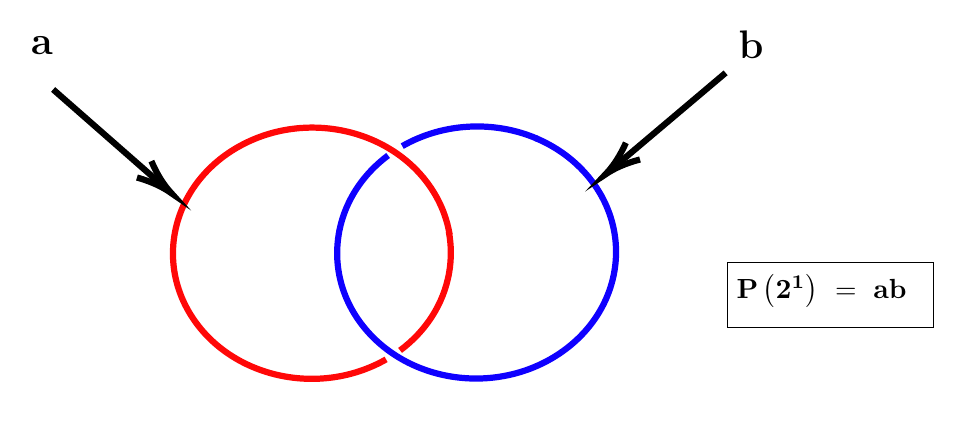
\begin{tikzpicture}[x=0.75pt,y=0.75pt,yscale=-1,xscale=1]
%uncomment if require: \path (0,300); %set diagram left start at 0, and has height of 300

%Shape: Arc [id:dp9265205120423934] 
\draw  [draw opacity=0][line width=2.25]  (293.28,103.86) .. controls (302.63,107.73) and (311.13,113.62) .. (317.93,121.44) .. controls (340.79,147.76) and (335.65,185.93) .. (306.43,206.71) .. controls (277.21,227.49) and (234.99,223) .. (212.12,196.69) .. controls (189.57,170.74) and (194.26,133.26) .. (222.4,112.3) -- (265.02,159.06) -- cycle ; \draw  [color={rgb, 255:red, 15; green, 0; blue, 255 }  ,draw opacity=1 ][line width=2.25]  (293.28,103.86) .. controls (302.63,107.73) and (311.13,113.62) .. (317.93,121.44) .. controls (340.79,147.76) and (335.65,185.93) .. (306.43,206.71) .. controls (277.21,227.49) and (234.99,223) .. (212.12,196.69) .. controls (189.57,170.74) and (194.26,133.26) .. (222.4,112.3) ;  
%Shape: Arc [id:dp8027414659974357] 
\draw  [draw opacity=0][line width=2.25]  (221.41,210.55) .. controls (220.57,211.03) and (219.72,211.49) .. (218.85,211.94) .. controls (186.68,228.52) and (145.79,218.45) .. (127.5,189.43) .. controls (109.21,160.41) and (120.46,123.44) .. (152.62,106.86) .. controls (184.78,90.27) and (225.68,100.35) .. (243.97,129.37) .. controls (248.23,136.12) and (250.88,143.31) .. (252.05,150.56) -- (185.73,159.4) -- cycle ; \draw  [color={rgb, 255:red, 255; green, 8; blue, 8 }  ,draw opacity=1 ][line width=2.25]  (221.41,210.55) .. controls (220.57,211.03) and (219.72,211.49) .. (218.85,211.94) .. controls (186.68,228.52) and (145.79,218.45) .. (127.5,189.43) .. controls (109.21,160.41) and (120.46,123.44) .. (152.62,106.86) .. controls (184.78,90.27) and (225.68,100.35) .. (243.97,129.37) .. controls (248.23,136.12) and (250.88,143.31) .. (252.05,150.56) ;  
%Shape: Arc [id:dp23180154013113696] 
\draw  [draw opacity=0][line width=2.25]  (229.2,107.81) .. controls (248.81,96.53) and (273.44,95.3) .. (294.07,104.17) -- (265.02,159.06) -- cycle ; \draw  [color={rgb, 255:red, 15; green, 0; blue, 255 }  ,draw opacity=1 ][line width=2.25]  (229.2,107.81) .. controls (248.81,96.53) and (273.44,95.3) .. (294.07,104.17) ;  
%Shape: Arc [id:dp9670832997214055] 
\draw  [draw opacity=0][line width=2.25]  (251.63,148.95) .. controls (252.87,155.4) and (252.96,162.14) .. (251.75,168.97) .. controls (249.05,184.18) and (240.33,197.16) .. (228.15,206.22) -- (185.73,159.4) -- cycle ; \draw  [color={rgb, 255:red, 255; green, 8; blue, 8 }  ,draw opacity=1 ][line width=2.25]  (251.63,148.95) .. controls (252.87,155.4) and (252.96,162.14) .. (251.75,168.97) .. controls (249.05,184.18) and (240.33,197.16) .. (228.15,206.22) ;  
%Straight Lines [id:da907333893615876] 
\draw [line width=2.25]    (61,80.5) -- (114.99,127.86) ;
\draw [shift={(118,130.5)}, rotate = 221.26] [color={rgb, 255:red, 0; green, 0; blue, 0 }  ][line width=2.25]    (17.49,-5.26) .. controls (11.12,-2.23) and (5.29,-0.48) .. (0,0) .. controls (5.29,0.48) and (11.12,2.23) .. (17.49,5.26)   ;
%Straight Lines [id:da8490006174497731] 
\draw [line width=2.25]    (385,72.5) -- (330.06,118.92) ;
\draw [shift={(327,121.5)}, rotate = 319.81] [color={rgb, 255:red, 0; green, 0; blue, 0 }  ][line width=2.25]    (17.49,-5.26) .. controls (11.12,-2.23) and (5.29,-0.48) .. (0,0) .. controls (5.29,0.48) and (11.12,2.23) .. (17.49,5.26)   ;

% Text Node
\draw (49,54) node [anchor=north west][inner sep=0.75pt]  [font=\Large] [align=left] {\textbf{a}};
% Text Node
\draw (390,51) node [anchor=north west][inner sep=0.75pt]  [font=\Large] [align=left] {\textbf{b}};
% Text Node
\draw    (386,164) -- (485,164) -- (485,195) -- (386,195) -- cycle  ;
\draw (389,168.4) node [anchor=north west][inner sep=0.75pt]    {$\mathbf{P\left( 2^{1}\right) \ =\ ab}$};


\end{tikzpicture}
}}
		\end{figure}
	\end{frame}
	\begin{frame}{\textbf{Polynomial Approach to Entanglement}}
		\begin{itemize}
			\item \onslide<2->{ There must not be any repeated terms, i.e., no ring
            variable can have a power greater than 1, eg aac is not valid as a has power 2.}
			\item \onslide<3->{Each ring variable must appear at least once, eg in a system of 4 qubits(a,b,c,d), abc+ab is not a valid polynomial, as d does not appear.}
			\item \onslide<4->{There must not be first-order terms, eg a + c is not valid.}.
			\item \onslide<5->{ Relabeling of variables is irrelevant, eg ab + abc and ac + abc represent same link.}
			\item \onslide<6->{ An n-variable monomial M is irrelevant if all of its variables are already present as an n-ring link of lesser-order  monomials, built only with the variables of M, eg ab + bc + abc is not valid as abc is irrelevant here. }
		\end{itemize}
	\end{frame}
	\begin{frame}{\textbf{Obtaining a Link from given State}}
		\begin{itemize}
			\item \onslide<2->{Given a state $\ket{\psi}$, we first check the entanglement property of the entire system using the Peres-Horodecki criterion.}
			\item \onslide<3->{We then calculate the partials traces of the density operator with respect to each system and then apply the PPT test. }
			\item \onslide<4->{From this, we can construct a link polynomial which is characterised by the given state. }
		\end{itemize}		
	\end{frame}
	\begin{frame}{\textbf{Obtaining State from a given Link}}
		\begin{itemize}
			\item \onslide<2->{In general, difficult to obtain state, given a link polynomial.}
			\item \onslide<3->{Given $\mathrm{N}$ qubits, there are $2^N$ basis states, namely $\ket{0}, \ket{1}, \ldots \ket{2^N-1}$}
			\item \onslide<4->{An algorithm has been devised to obtain a general structure of the state from the link.} 
			\item \onslide<5->{But it only produces a mixed state only \Sadey \ !}
		\end{itemize}
		\onslide<6->{\textbf{Algorithm:}}
		\begin{enumerate}
			\item \onslide<7->{Take a term $t$ of the link polynomial $P(\{t\})$}
			\item \onslide<8->{$t$  mapped to a state: $\ket{\mathrm{E_q}}\otimes\ket{\mathrm{S_q}}\otimes\ket{\mathrm{Q_d}}$}
			\begin{itemize}
				\onslide<9->{\item $\ket{\mathrm{E_q}}\longrightarrow $ entangled qubit of GHZ type, associated to ring variables in $t$.}
				\onslide<10->{\item $\ket{\mathrm{S_q}}\longrightarrow$ separable qubit associated with ring variables not in $t$. Generally, large number of possibilities for this separable qubit.}
				\onslide<11->{\item $\ket{\mathrm{Q_d}}\longrightarrow$  qudit state associated with \textit{artifically} introduced ring variable (alphabetical successor of the largest ring variable present). To be traced out later, hence is of less significance. Can be a random state, hence it becomes \textbf{mixed}. }
			\end{itemize}
			\item \onslide<12->{Full state $\ket{\psi}\longrightarrow$ sum of individual such states. Trace out $d$ and obtain density matrix of reduced system.}
		\end{enumerate}
		
	\end{frame}
	\begin{frame}{\textbf{Demonstration of Algorithm}}
	\onslide<2->{Let us take a look at a demonstration of the algorithm. Take: $$\mathcolor{red}{\mathrm{P(a,b,c)=ab+ac}}$$}
		\begin{itemize}
			\item \onslide<3->{Choose the term $t=ab$}
			\item \onslide<4->{Two ring variables $a$ and $b$, so 2 qubit GHZ state assigned to entangled part. $\ket{\mathrm{E_q}} = \frac{1}{\sqrt{2}}\brac{\ket{00} + \ket{11}}\equiv \ket{2^1}_{ab}$}
			\item \onslide<5->{Separable qubit associated with $c$, keep it general $\ket{\mathrm{S_q}} = \ket{q_1}_c$}
			\item \onslide<6->{Qudit state, take $\ket{\mathrm{Q_d}}= \ket{0}_d$ }
			\item \onslide<7->{\textbf{Full state becomes}: $$\ket{\psi_1} = \ket{2^1}_{ab}\otimes\ket{q_1}_c\otimes\ket{0}_d $$}

		\end{itemize}
		

	\end{frame}





	\begin{frame}{\textbf{Demonstration of Algorithm}}
		\onslide<1->{Let us take a look at a demonstration of the algorithm. Take: $$\mathcolor{red}{\mathrm{P(a,b,c)=ab+ac}}$$}
			\begin{itemize}
			\item \onslide<1->{Choose the term $t=ac$}
				\item \onslide<2->{Two ring variables $a$ and $c$, so 2 qubit GHZ state assigned to entangled part. $\ket{\mathrm{E_q}} = \frac{1}{\sqrt{2}}\brac{\ket{00} + \ket{11}}\equiv \ket{2^1}_{ac}$}
				\item \onslide<3->{Separable qubit associated with $b$, keep it general $\ket{\mathrm{S_q}} = \ket{q_1}_b$}
				\item \onslide<4->{Qudit state, take $\ket{\mathrm{Q_d}}= \ket{1}_d$ }
				\item \onslide<5->{\textbf{Full state becomes}: $\ket{\psi_2} = \ket{2^1}_{ac}\otimes\ket{q_2}_b\otimes\ket{1}_d$}
			\end{itemize}
		\end{frame}
		\begin{frame}{Demonstration of Algorithm}

			\begin{itemize}
				\item \onslide<1->{\textbf{Mixed state characterising the link}: $ \ket{\psi} = c_1\ket{\psi_1} + c_2\ket{\psi_2}$}
				\item \onslide<2->{ Then construct the density matrix accordingly for the state. }
			\end{itemize}
			\begin{figure}
				\centering 
				\scalebox{0.6}{

\tikzset{every picture/.style={line width=0.75pt}} %set default line width to 0.75pt        

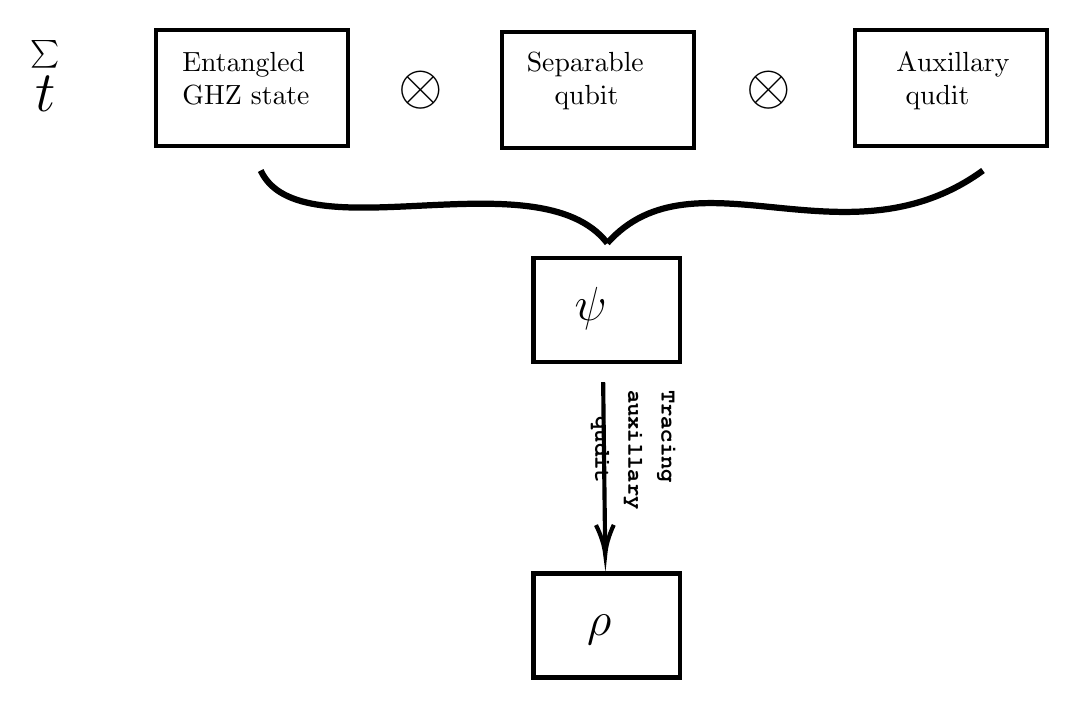
\begin{tikzpicture}[x=0.75pt,y=0.75pt,yscale=-1,xscale=1]
%uncomment if require: \path (0,418); %set diagram left start at 0, and has height of 418

%Shape: Rectangle [id:dp7294540182578855] 
\draw  [color={rgb, 255:red, 0; green, 0; blue, 0 }  ,draw opacity=1 ][fill={rgb, 255:red, 255; green, 255; blue, 255 }  ,fill opacity=1 ][line width=1.5]  (86.44,31.57) -- (178.88,31.57) -- (178.88,87.63) -- (86.44,87.63) -- cycle ;
%Shape: Rectangle [id:dp4761246648053713] 
\draw  [color={rgb, 255:red, 0; green, 0; blue, 0 }  ,draw opacity=1 ][fill={rgb, 255:red, 255; green, 255; blue, 255 }  ,fill opacity=1 ][line width=1.5]  (253.44,32.57) -- (345.88,32.57) -- (345.88,88.63) -- (253.44,88.63) -- cycle ;
%Shape: Rectangle [id:dp5375732459667567] 
\draw  [color={rgb, 255:red, 0; green, 0; blue, 0 }  ,draw opacity=1 ][fill={rgb, 255:red, 255; green, 255; blue, 255 }  ,fill opacity=1 ][line width=1.5]  (423.44,31.57) -- (515.88,31.57) -- (515.88,87.63) -- (423.44,87.63) -- cycle ;
%Shape: Rectangle [id:dp8708856606447273] 
\draw  [color={rgb, 255:red, 0; green, 0; blue, 0 }  ,draw opacity=1 ][fill={rgb, 255:red, 255; green, 255; blue, 255 }  ,fill opacity=1 ][line width=1.5]  (268.44,141.57) -- (339,141.57) -- (339,191.62) -- (268.44,191.62) -- cycle ;
%Curve Lines [id:da5387806644578281] 
\draw [line width=2.25]    (137,99.38) .. controls (156,140.38) and (271,91.77) .. (304,134.38) ;
%Curve Lines [id:da3604580216133906] 
\draw [line width=2.25]    (304,134.38) .. controls (346,87.38) and (419,147.38) .. (485,99.38) ;
%Straight Lines [id:da04531485758321774] 
\draw [line width=1.5]    (302,201.38) -- (302.96,281.38) ;
\draw [shift={(303,284.38)}, rotate = 269.31] [color={rgb, 255:red, 0; green, 0; blue, 0 }  ][line width=1.5]    (14.21,-4.28) .. controls (9.04,-1.82) and (4.3,-0.39) .. (0,0) .. controls (4.3,0.39) and (9.04,1.82) .. (14.21,4.28)   ;
%Shape: Rectangle [id:dp4350486178723396] 
\draw  [color={rgb, 255:red, 0; green, 0; blue, 0 }  ,draw opacity=1 ][fill={rgb, 255:red, 255; green, 255; blue, 255 }  ,fill opacity=1 ][line width=1.5]  (268.44,293.57) -- (339,293.57) -- (339,343.62) -- (268.44,343.62) -- cycle ;

% Text Node
\draw (97.98,41) node [anchor=north west][inner sep=0.75pt]   [align=left] {Entangled\\GHZ state};
% Text Node
\draw (263.98,41) node [anchor=north west][inner sep=0.75pt]   [align=left] {Separable\\ \ \ \ qubit};
% Text Node
\draw (441.98,41) node [anchor=north west][inner sep=0.75pt]   [align=left] {Auxillary \\ \ qudit};
% Text Node
\draw (287,154.4) node [anchor=north west][inner sep=0.75pt]  [font=\LARGE]  {$\ket{\psi }$};
% Text Node
\draw (202,50.4) node [anchor=north west][inner sep=0.75pt]  [font=\huge]  {$\mathlarger{\otimes} $};
% Text Node
\draw (370,50) node [anchor=north west][inner sep=0.75pt]  [font=\huge]  {$\mathbf{\otimes} $};
% Text Node
\draw (293,312.4) node [anchor=north west][inner sep=0.75pt]  [font=\LARGE]  {$\rho $};
% Text Node
\draw (338.5,203.88) node [anchor=north west][inner sep=0.75pt]  [rotate=-90] [align=left] {{\footnotesize {\fontfamily{pcr}\selectfont  \textbf{Tracing} }}\\{\footnotesize {\fontfamily{pcr}\selectfont \textbf{auxillary}}}\\{\footnotesize {\fontfamily{pcr}\selectfont  \ \ \textbf{qudit}}}};
% Text Node
\draw (25,35.4) node [anchor=north west][inner sep=0.75pt]  [font=\Huge]  {$\sum \limits_{{t}}$};


\end{tikzpicture}
}
				\caption{Schematic representation of the algorithm.}
			\end{figure}
			
		\end{frame}
	\begin{frame}
		\begin{center}
			\textbf{\Huge Some Examples...}
		\end{center}
	\end{frame}
	\begin{frame}{\textbf{Three Qubit System}: 3\textsuperscript{1} class}
		\onslide<1->{\textcolor{red}{\textbf{Pure State:} } $\ket{3^1}_{abc} = \frac{1}{\sqrt{2}}\brac{\ket{000}_{abc}+\ket{111}_{abc}}$}\\[0.3cm]
		
		\onslide<2->{\begin{minipage}{0.35\textwidth}
			%

\tikzset{every picture/.style={line width=0.75pt}} %set default line width to 0.75pt        

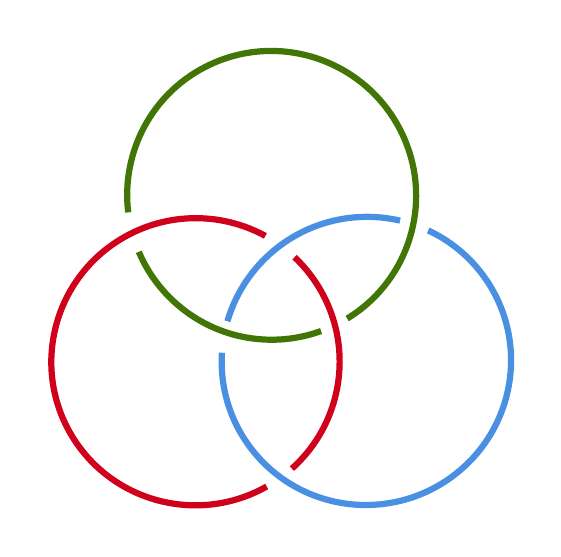
\begin{tikzpicture}[x=0.75pt,y=0.75pt,yscale=-1,xscale=1]
%uncomment if require: \path (0,300); %set diagram left start at 0, and has height of 300

%Shape: Arc [id:dp49278097545949884] 
\draw  [draw opacity=0][line width=2.25]  (328.62,163.73) .. controls (321.19,166.44) and (313.18,167.92) .. (304.82,167.92) .. controls (276.06,167.92) and (251.39,150.46) .. (240.8,125.56) -- (304.82,98.33) -- cycle ; \draw  [color={rgb, 255:red, 65; green, 117; blue, 5 }  ,draw opacity=1 ][line width=2.25]  (328.62,163.73) .. controls (321.19,166.44) and (313.18,167.92) .. (304.82,167.92) .. controls (276.06,167.92) and (251.39,150.46) .. (240.8,125.56) ;  
%Shape: Arc [id:dp7313937278600963] 
\draw  [draw opacity=0][line width=2.25]  (380.22,115.26) .. controls (389.75,119.69) and (398.4,126.36) .. (405.34,135.15) .. controls (429.07,165.23) and (423.73,208.87) .. (393.41,232.62) .. controls (363.09,256.37) and (319.27,251.24) .. (295.54,221.15) .. controls (284.6,207.29) and (279.84,190.54) .. (280.85,174.18) -- (350.44,178.15) -- cycle ; \draw  [color={rgb, 255:red, 74; green, 144; blue, 226 }  ,draw opacity=1 ][line width=2.25]  (380.22,115.26) .. controls (389.75,119.69) and (398.4,126.36) .. (405.34,135.15) .. controls (429.07,165.23) and (423.73,208.87) .. (393.41,232.62) .. controls (363.09,256.37) and (319.27,251.24) .. (295.54,221.15) .. controls (284.6,207.29) and (279.84,190.54) .. (280.85,174.18) ;  
%Shape: Arc [id:dp9082888658781946] 
\draw  [draw opacity=0][line width=2.25]  (235.71,106.58) .. controls (232.15,77.58) and (247.26,48.37) .. (275.16,35.34) .. controls (309.93,19.08) and (351.4,34.11) .. (367.78,68.91) .. controls (383.06,101.37) and (371.11,139.56) .. (341.2,157.73) -- (304.82,98.33) -- cycle ; \draw  [color={rgb, 255:red, 65; green, 117; blue, 5 }  ,draw opacity=1 ][line width=2.25]  (235.71,106.58) .. controls (232.15,77.58) and (247.26,48.37) .. (275.16,35.34) .. controls (309.93,19.08) and (351.4,34.11) .. (367.78,68.91) .. controls (383.06,101.37) and (371.11,139.56) .. (341.2,157.73) ;  
%Shape: Arc [id:dp7357603003827937] 
\draw  [draw opacity=0][line width=2.25]  (302.44,238.64) .. controls (269.08,257.52) and (226.71,245.99) .. (207.75,212.86) .. controls (188.77,179.69) and (200.44,137.44) .. (233.81,118.48) .. controls (255.62,106.09) and (281.32,106.72) .. (301.8,117.92) -- (268.17,178.53) -- cycle ; \draw  [color={rgb, 255:red, 208; green, 2; blue, 27 }  ,draw opacity=1 ][line width=2.25]  (302.44,238.64) .. controls (269.08,257.52) and (226.71,245.99) .. (207.75,212.86) .. controls (188.77,179.69) and (200.44,137.44) .. (233.81,118.48) .. controls (255.62,106.09) and (281.32,106.72) .. (301.8,117.92) ;  
%Shape: Arc [id:dp02993817280793909] 
\draw  [draw opacity=0][line width=2.25]  (283.51,159.01) .. controls (286.66,148.19) and (292.5,137.97) .. (301.03,129.39) .. controls (318.8,111.52) and (343.85,105.22) .. (366.69,110.55) -- (350.44,178.15) -- cycle ; \draw  [color={rgb, 255:red, 74; green, 144; blue, 226 }  ,draw opacity=1 ][line width=2.25]  (283.51,159.01) .. controls (286.66,148.19) and (292.5,137.97) .. (301.03,129.39) .. controls (318.8,111.52) and (343.85,105.22) .. (366.69,110.55) ;  
%Shape: Arc [id:dp6464277844327507] 
\draw  [draw opacity=0][line width=2.25]  (315.85,128.16) .. controls (331.94,143.37) and (340.46,165.99) .. (336.68,189.48) .. controls (334.06,205.76) and (325.96,219.8) .. (314.56,230.03) -- (268.17,178.53) -- cycle ; \draw  [color={rgb, 255:red, 208; green, 2; blue, 27 }  ,draw opacity=1 ][line width=2.25]  (315.85,128.16) .. controls (331.94,143.37) and (340.46,165.99) .. (336.68,189.48) .. controls (334.06,205.76) and (325.96,219.8) .. (314.56,230.03) ;  




\end{tikzpicture}
  % Make sure this file exists
			\scalebox{0.6}{

\tikzset{every picture/.style={line width=0.75pt}} %set default line width to 0.75pt        

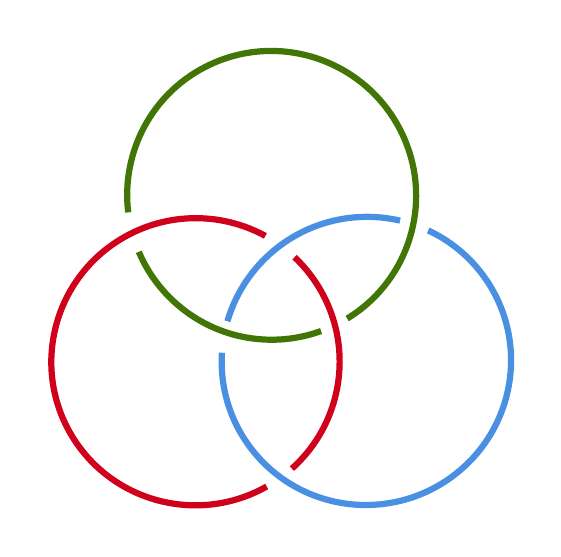
\begin{tikzpicture}[x=0.75pt,y=0.75pt,yscale=-1,xscale=1]
%uncomment if require: \path (0,300); %set diagram left start at 0, and has height of 300

%Shape: Arc [id:dp49278097545949884] 
\draw  [draw opacity=0][line width=2.25]  (328.62,163.73) .. controls (321.19,166.44) and (313.18,167.92) .. (304.82,167.92) .. controls (276.06,167.92) and (251.39,150.46) .. (240.8,125.56) -- (304.82,98.33) -- cycle ; \draw  [color={rgb, 255:red, 65; green, 117; blue, 5 }  ,draw opacity=1 ][line width=2.25]  (328.62,163.73) .. controls (321.19,166.44) and (313.18,167.92) .. (304.82,167.92) .. controls (276.06,167.92) and (251.39,150.46) .. (240.8,125.56) ;  
%Shape: Arc [id:dp7313937278600963] 
\draw  [draw opacity=0][line width=2.25]  (380.22,115.26) .. controls (389.75,119.69) and (398.4,126.36) .. (405.34,135.15) .. controls (429.07,165.23) and (423.73,208.87) .. (393.41,232.62) .. controls (363.09,256.37) and (319.27,251.24) .. (295.54,221.15) .. controls (284.6,207.29) and (279.84,190.54) .. (280.85,174.18) -- (350.44,178.15) -- cycle ; \draw  [color={rgb, 255:red, 74; green, 144; blue, 226 }  ,draw opacity=1 ][line width=2.25]  (380.22,115.26) .. controls (389.75,119.69) and (398.4,126.36) .. (405.34,135.15) .. controls (429.07,165.23) and (423.73,208.87) .. (393.41,232.62) .. controls (363.09,256.37) and (319.27,251.24) .. (295.54,221.15) .. controls (284.6,207.29) and (279.84,190.54) .. (280.85,174.18) ;  
%Shape: Arc [id:dp9082888658781946] 
\draw  [draw opacity=0][line width=2.25]  (235.71,106.58) .. controls (232.15,77.58) and (247.26,48.37) .. (275.16,35.34) .. controls (309.93,19.08) and (351.4,34.11) .. (367.78,68.91) .. controls (383.06,101.37) and (371.11,139.56) .. (341.2,157.73) -- (304.82,98.33) -- cycle ; \draw  [color={rgb, 255:red, 65; green, 117; blue, 5 }  ,draw opacity=1 ][line width=2.25]  (235.71,106.58) .. controls (232.15,77.58) and (247.26,48.37) .. (275.16,35.34) .. controls (309.93,19.08) and (351.4,34.11) .. (367.78,68.91) .. controls (383.06,101.37) and (371.11,139.56) .. (341.2,157.73) ;  
%Shape: Arc [id:dp7357603003827937] 
\draw  [draw opacity=0][line width=2.25]  (302.44,238.64) .. controls (269.08,257.52) and (226.71,245.99) .. (207.75,212.86) .. controls (188.77,179.69) and (200.44,137.44) .. (233.81,118.48) .. controls (255.62,106.09) and (281.32,106.72) .. (301.8,117.92) -- (268.17,178.53) -- cycle ; \draw  [color={rgb, 255:red, 208; green, 2; blue, 27 }  ,draw opacity=1 ][line width=2.25]  (302.44,238.64) .. controls (269.08,257.52) and (226.71,245.99) .. (207.75,212.86) .. controls (188.77,179.69) and (200.44,137.44) .. (233.81,118.48) .. controls (255.62,106.09) and (281.32,106.72) .. (301.8,117.92) ;  
%Shape: Arc [id:dp02993817280793909] 
\draw  [draw opacity=0][line width=2.25]  (283.51,159.01) .. controls (286.66,148.19) and (292.5,137.97) .. (301.03,129.39) .. controls (318.8,111.52) and (343.85,105.22) .. (366.69,110.55) -- (350.44,178.15) -- cycle ; \draw  [color={rgb, 255:red, 74; green, 144; blue, 226 }  ,draw opacity=1 ][line width=2.25]  (283.51,159.01) .. controls (286.66,148.19) and (292.5,137.97) .. (301.03,129.39) .. controls (318.8,111.52) and (343.85,105.22) .. (366.69,110.55) ;  
%Shape: Arc [id:dp6464277844327507] 
\draw  [draw opacity=0][line width=2.25]  (315.85,128.16) .. controls (331.94,143.37) and (340.46,165.99) .. (336.68,189.48) .. controls (334.06,205.76) and (325.96,219.8) .. (314.56,230.03) -- (268.17,178.53) -- cycle ; \draw  [color={rgb, 255:red, 208; green, 2; blue, 27 }  ,draw opacity=1 ][line width=2.25]  (315.85,128.16) .. controls (331.94,143.37) and (340.46,165.99) .. (336.68,189.48) .. controls (334.06,205.76) and (325.96,219.8) .. (314.56,230.03) ;  




\end{tikzpicture}
}
			\begin{itemize}
				\onslide<5->{\item \textbf{Eigenvalues:} $0.0,\ 0.5,\ \mathcolor{red}{-0.5}$}
				\onslide<6->{\item One eigenvalue is negative $\rightarrow$ \textbf{\textcolor{OliveGreen}{Tripartite Entanglement}}}
			\end{itemize}
		\end{minipage}}%
		\onslide<3->{\begin{minipage}{0.5\textwidth}
			\footnotesize
			\begin{equation*}
				\rho_{abc} =
				\left[
				\begin{array}{cccccccc}
				0.5 & 0.0 & 0.0 & 0.0 & 0.0 & 0.0 & 0.0 & 0.5 \\
				0.0 & 0.0 & 0.0 & 0.0 & 0.0 & 0.0 & 0.0 & 0.0 \\
				0.0 & 0.0 & 0.0 & 0.0 & 0.0 & 0.0 & 0.0 & 0.0 \\
				0.0 & 0.0 & 0.0 & 0.0 & 0.0 & 0.0 & 0.0 & 0.0 \\
				0.0 & 0.0 & 0.0 & 0.0 & 0.0 & 0.0 & 0.0 & 0.0 \\
				0.0 & 0.0 & 0.0 & 0.0 & 0.0 & 0.0 & 0.0 & 0.0 \\
				0.0 & 0.0 & 0.0 & 0.0 & 0.0 & 0.0 & 0.0 & 0.0 \\
				0.5 & 0.0 & 0.0 & 0.0 & 0.0 & 0.0 & 0.0 & 0.5 \\
				\end{array}
				\right]
			\end{equation*}}
			\onslide<4->{\begin{equation*}
				\rho^{T_a}_{abc} =
				\left[
				\begin{array}{cccccccc}
				0.5 & 0.0 & 0.0 & 0.0 & 0.0 & 0.0 & 0.0 & 0.0 \\
				0.0 & 0.0 & 0.0 & 0.0 & 0.0 & 0.0 & 0.0 & 0.0 \\
				0.0 & 0.0 & 0.0 & 0.0 & 0.0 & 0.0 & 0.0 & 0.0 \\
				0.0 & 0.0 & 0.0 & 0.0 & 0.5 & 0.0 & 0.0 & 0.0 \\
				0.0 & 0.0 & 0.0 & 0.5 & 0.0 & 0.0 & 0.0 & 0.0 \\
				0.0 & 0.0 & 0.0 & 0.0 & 0.0 & 0.0 & 0.0 & 0.0 \\
				0.0 & 0.0 & 0.0 & 0.0 & 0.0 & 0.0 & 0.0 & 0.0 \\
				0.0 & 0.0 & 0.0 & 0.0 & 0.0 & 0.0 & 0.0 & 0.5 \\
				\end{array}
				\right]
				\end{equation*}
		\end{minipage}}
	\end{frame}
	\begin{frame}{\textbf{Three Qubit System}: 3\textsuperscript{1} class}
		\onslide<1->{\textcolor{red}{\textbf{Pure State:} } $\ket{3^1}_{abc} = \frac{1}{\sqrt{2}}\brac{\ket{000}_{abc}+\ket{111}_{abc}}$}\\[0.3cm]
		\begin{minipage}{0.35\textwidth}
			%

\tikzset{every picture/.style={line width=0.75pt}} %set default line width to 0.75pt        

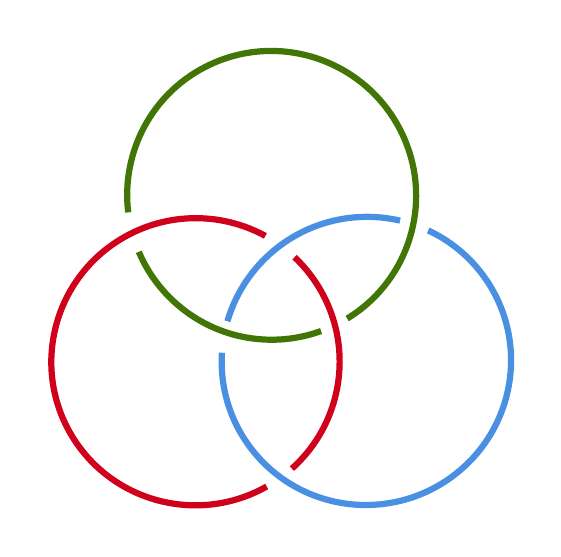
\begin{tikzpicture}[x=0.75pt,y=0.75pt,yscale=-1,xscale=1]
%uncomment if require: \path (0,300); %set diagram left start at 0, and has height of 300

%Shape: Arc [id:dp49278097545949884] 
\draw  [draw opacity=0][line width=2.25]  (328.62,163.73) .. controls (321.19,166.44) and (313.18,167.92) .. (304.82,167.92) .. controls (276.06,167.92) and (251.39,150.46) .. (240.8,125.56) -- (304.82,98.33) -- cycle ; \draw  [color={rgb, 255:red, 65; green, 117; blue, 5 }  ,draw opacity=1 ][line width=2.25]  (328.62,163.73) .. controls (321.19,166.44) and (313.18,167.92) .. (304.82,167.92) .. controls (276.06,167.92) and (251.39,150.46) .. (240.8,125.56) ;  
%Shape: Arc [id:dp7313937278600963] 
\draw  [draw opacity=0][line width=2.25]  (380.22,115.26) .. controls (389.75,119.69) and (398.4,126.36) .. (405.34,135.15) .. controls (429.07,165.23) and (423.73,208.87) .. (393.41,232.62) .. controls (363.09,256.37) and (319.27,251.24) .. (295.54,221.15) .. controls (284.6,207.29) and (279.84,190.54) .. (280.85,174.18) -- (350.44,178.15) -- cycle ; \draw  [color={rgb, 255:red, 74; green, 144; blue, 226 }  ,draw opacity=1 ][line width=2.25]  (380.22,115.26) .. controls (389.75,119.69) and (398.4,126.36) .. (405.34,135.15) .. controls (429.07,165.23) and (423.73,208.87) .. (393.41,232.62) .. controls (363.09,256.37) and (319.27,251.24) .. (295.54,221.15) .. controls (284.6,207.29) and (279.84,190.54) .. (280.85,174.18) ;  
%Shape: Arc [id:dp9082888658781946] 
\draw  [draw opacity=0][line width=2.25]  (235.71,106.58) .. controls (232.15,77.58) and (247.26,48.37) .. (275.16,35.34) .. controls (309.93,19.08) and (351.4,34.11) .. (367.78,68.91) .. controls (383.06,101.37) and (371.11,139.56) .. (341.2,157.73) -- (304.82,98.33) -- cycle ; \draw  [color={rgb, 255:red, 65; green, 117; blue, 5 }  ,draw opacity=1 ][line width=2.25]  (235.71,106.58) .. controls (232.15,77.58) and (247.26,48.37) .. (275.16,35.34) .. controls (309.93,19.08) and (351.4,34.11) .. (367.78,68.91) .. controls (383.06,101.37) and (371.11,139.56) .. (341.2,157.73) ;  
%Shape: Arc [id:dp7357603003827937] 
\draw  [draw opacity=0][line width=2.25]  (302.44,238.64) .. controls (269.08,257.52) and (226.71,245.99) .. (207.75,212.86) .. controls (188.77,179.69) and (200.44,137.44) .. (233.81,118.48) .. controls (255.62,106.09) and (281.32,106.72) .. (301.8,117.92) -- (268.17,178.53) -- cycle ; \draw  [color={rgb, 255:red, 208; green, 2; blue, 27 }  ,draw opacity=1 ][line width=2.25]  (302.44,238.64) .. controls (269.08,257.52) and (226.71,245.99) .. (207.75,212.86) .. controls (188.77,179.69) and (200.44,137.44) .. (233.81,118.48) .. controls (255.62,106.09) and (281.32,106.72) .. (301.8,117.92) ;  
%Shape: Arc [id:dp02993817280793909] 
\draw  [draw opacity=0][line width=2.25]  (283.51,159.01) .. controls (286.66,148.19) and (292.5,137.97) .. (301.03,129.39) .. controls (318.8,111.52) and (343.85,105.22) .. (366.69,110.55) -- (350.44,178.15) -- cycle ; \draw  [color={rgb, 255:red, 74; green, 144; blue, 226 }  ,draw opacity=1 ][line width=2.25]  (283.51,159.01) .. controls (286.66,148.19) and (292.5,137.97) .. (301.03,129.39) .. controls (318.8,111.52) and (343.85,105.22) .. (366.69,110.55) ;  
%Shape: Arc [id:dp6464277844327507] 
\draw  [draw opacity=0][line width=2.25]  (315.85,128.16) .. controls (331.94,143.37) and (340.46,165.99) .. (336.68,189.48) .. controls (334.06,205.76) and (325.96,219.8) .. (314.56,230.03) -- (268.17,178.53) -- cycle ; \draw  [color={rgb, 255:red, 208; green, 2; blue, 27 }  ,draw opacity=1 ][line width=2.25]  (315.85,128.16) .. controls (331.94,143.37) and (340.46,165.99) .. (336.68,189.48) .. controls (334.06,205.76) and (325.96,219.8) .. (314.56,230.03) ;  




\end{tikzpicture}
  % Make sure this file exists
			\onslide<2->{\scalebox{0.6}{

\tikzset{every picture/.style={line width=0.75pt}} %set default line width to 0.75pt        

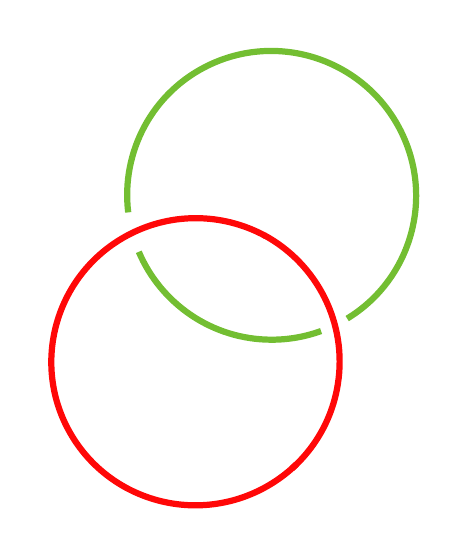
\begin{tikzpicture}[x=0.75pt,y=0.75pt,yscale=-1,xscale=1]
%uncomment if require: \path (0,300); %set diagram left start at 0, and has height of 300

%Shape: Arc [id:dp9961343423853242] 
\draw  [draw opacity=0][line width=2.25]  (348.62,177.2) .. controls (341.19,179.91) and (333.18,181.38) .. (324.82,181.38) .. controls (296.06,181.38) and (271.39,163.93) .. (260.8,139.03) -- (324.82,111.8) -- cycle ; \draw  [color={rgb, 255:red, 115; green, 190; blue, 50 }  ,draw opacity=1 ][line width=2.25]  (348.62,177.2) .. controls (341.19,179.91) and (333.18,181.38) .. (324.82,181.38) .. controls (296.06,181.38) and (271.39,163.93) .. (260.8,139.03) ;  
%Shape: Arc [id:dp11612154435512079] 
\draw  [draw opacity=0][line width=2.25]  (255.71,120.05) .. controls (252.15,91.05) and (267.26,61.84) .. (295.16,48.8) .. controls (329.93,32.55) and (371.4,47.58) .. (387.78,82.37) .. controls (403.06,114.84) and (391.11,153.03) .. (361.2,171.2) -- (324.82,111.8) -- cycle ; \draw  [color={rgb, 255:red, 115; green, 190; blue, 50 }  ,draw opacity=1 ][line width=2.25]  (255.71,120.05) .. controls (252.15,91.05) and (267.26,61.84) .. (295.16,48.8) .. controls (329.93,32.55) and (371.4,47.58) .. (387.78,82.37) .. controls (403.06,114.84) and (391.11,153.03) .. (361.2,171.2) ;  
%Shape: Arc [id:dp5786194174920847] 
\draw  [draw opacity=0][line width=2.25]  (336.8,241.34) .. controls (332.62,245.42) and (327.85,249.03) .. (322.53,252.05) .. controls (289.16,271.01) and (246.73,259.49) .. (227.75,226.32) .. controls (208.77,193.16) and (220.44,150.91) .. (253.81,131.95) .. controls (275.62,119.56) and (301.32,120.19) .. (321.8,131.39) -- (288.17,192) -- cycle ; \draw  [color={rgb, 255:red, 255; green, 8; blue, 8 }  ,draw opacity=1 ][line width=2.25]  (336.8,241.34) .. controls (332.62,245.42) and (327.85,249.03) .. (322.53,252.05) .. controls (289.16,271.01) and (246.73,259.49) .. (227.75,226.32) .. controls (208.77,193.16) and (220.44,150.91) .. (253.81,131.95) .. controls (275.62,119.56) and (301.32,120.19) .. (321.8,131.39) ;  
%Shape: Arc [id:dp2668566217368272] 
\draw  [draw opacity=0][line width=2.25]  (321.26,131.06) .. controls (346.43,144.68) and (361.48,173.11) .. (356.68,202.95) .. controls (354.06,219.23) and (345.96,233.27) .. (334.56,243.5) -- (288.17,192) -- cycle ; \draw  [color={rgb, 255:red, 255; green, 8; blue, 8 }  ,draw opacity=1 ][line width=2.25]  (321.26,131.06) .. controls (346.43,144.68) and (361.48,173.11) .. (356.68,202.95) .. controls (354.06,219.23) and (345.96,233.27) .. (334.56,243.5) ;  




\end{tikzpicture}
}}
			\begin{itemize}
				\onslide<5->{\item \textbf{Eigenvalues:} $0.0,\ 0.5\geq0$}
			\end{itemize}
		\end{minipage}%
		\begin{minipage}{0.5\textwidth}
			\footnotesize
			\onslide<3->{\begin{equation*}
				\rho_{ab}
				\left[
				\begin{array}{cccc}
				0.5 & 0.0 & 0.0 & 0.0 \\
				0.0 & 0.0 & 0.0 & 0.0 \\
				0.0 & 0.0 & 0.0 & 0.0 \\
				0.0 & 0.0 & 0.0 & 0.5 \\
				\end{array}
				\right]
				\end{equation*} }
				\onslide<4->{\begin{equation*}
					\rho^{Ta}_{ab}
					\left[
					\begin{array}{cccc}
					0.5 & 0.0 & 0.0 & 0.0 \\
					0.0 & 0.0 & 0.0 & 0.0 \\
					0.0 & 0.0 & 0.0 & 0.0 \\
					0.0 & 0.0 & 0.0 & 0.5 \\
					\end{array}
					\right]
					\end{equation*}}
				\begin{itemize}
					\onslide<6->{\item All eigenvalues are positive.}
					\onslide<7->{\item System completely \textbf{separable} after cut.}
				\end{itemize}
		\end{minipage}
	\end{frame}





	\begin{frame}{\textbf{Three Qubit System}: 3\textsuperscript{2} class}
		\onslide<1->{\textcolor{red}{\textbf{Pure State:} } $\ket{3^2}_{abc} = \frac{1}{\sqrt{3}}\brac{\ket{000}_{abc} + \ket{111}_{abc} + \ket{001}_{abc}}} $\\[0.3cm]
		\begin{minipage}{0.35\textwidth}
			%

\tikzset{every picture/.style={line width=0.75pt}} %set default line width to 0.75pt        

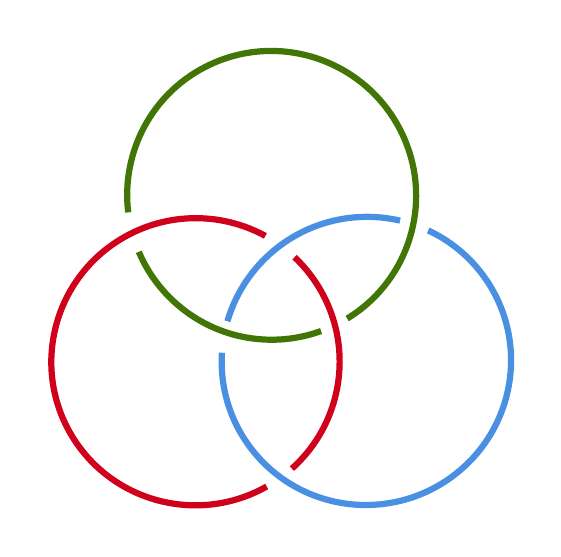
\begin{tikzpicture}[x=0.75pt,y=0.75pt,yscale=-1,xscale=1]
%uncomment if require: \path (0,300); %set diagram left start at 0, and has height of 300

%Shape: Arc [id:dp49278097545949884] 
\draw  [draw opacity=0][line width=2.25]  (328.62,163.73) .. controls (321.19,166.44) and (313.18,167.92) .. (304.82,167.92) .. controls (276.06,167.92) and (251.39,150.46) .. (240.8,125.56) -- (304.82,98.33) -- cycle ; \draw  [color={rgb, 255:red, 65; green, 117; blue, 5 }  ,draw opacity=1 ][line width=2.25]  (328.62,163.73) .. controls (321.19,166.44) and (313.18,167.92) .. (304.82,167.92) .. controls (276.06,167.92) and (251.39,150.46) .. (240.8,125.56) ;  
%Shape: Arc [id:dp7313937278600963] 
\draw  [draw opacity=0][line width=2.25]  (380.22,115.26) .. controls (389.75,119.69) and (398.4,126.36) .. (405.34,135.15) .. controls (429.07,165.23) and (423.73,208.87) .. (393.41,232.62) .. controls (363.09,256.37) and (319.27,251.24) .. (295.54,221.15) .. controls (284.6,207.29) and (279.84,190.54) .. (280.85,174.18) -- (350.44,178.15) -- cycle ; \draw  [color={rgb, 255:red, 74; green, 144; blue, 226 }  ,draw opacity=1 ][line width=2.25]  (380.22,115.26) .. controls (389.75,119.69) and (398.4,126.36) .. (405.34,135.15) .. controls (429.07,165.23) and (423.73,208.87) .. (393.41,232.62) .. controls (363.09,256.37) and (319.27,251.24) .. (295.54,221.15) .. controls (284.6,207.29) and (279.84,190.54) .. (280.85,174.18) ;  
%Shape: Arc [id:dp9082888658781946] 
\draw  [draw opacity=0][line width=2.25]  (235.71,106.58) .. controls (232.15,77.58) and (247.26,48.37) .. (275.16,35.34) .. controls (309.93,19.08) and (351.4,34.11) .. (367.78,68.91) .. controls (383.06,101.37) and (371.11,139.56) .. (341.2,157.73) -- (304.82,98.33) -- cycle ; \draw  [color={rgb, 255:red, 65; green, 117; blue, 5 }  ,draw opacity=1 ][line width=2.25]  (235.71,106.58) .. controls (232.15,77.58) and (247.26,48.37) .. (275.16,35.34) .. controls (309.93,19.08) and (351.4,34.11) .. (367.78,68.91) .. controls (383.06,101.37) and (371.11,139.56) .. (341.2,157.73) ;  
%Shape: Arc [id:dp7357603003827937] 
\draw  [draw opacity=0][line width=2.25]  (302.44,238.64) .. controls (269.08,257.52) and (226.71,245.99) .. (207.75,212.86) .. controls (188.77,179.69) and (200.44,137.44) .. (233.81,118.48) .. controls (255.62,106.09) and (281.32,106.72) .. (301.8,117.92) -- (268.17,178.53) -- cycle ; \draw  [color={rgb, 255:red, 208; green, 2; blue, 27 }  ,draw opacity=1 ][line width=2.25]  (302.44,238.64) .. controls (269.08,257.52) and (226.71,245.99) .. (207.75,212.86) .. controls (188.77,179.69) and (200.44,137.44) .. (233.81,118.48) .. controls (255.62,106.09) and (281.32,106.72) .. (301.8,117.92) ;  
%Shape: Arc [id:dp02993817280793909] 
\draw  [draw opacity=0][line width=2.25]  (283.51,159.01) .. controls (286.66,148.19) and (292.5,137.97) .. (301.03,129.39) .. controls (318.8,111.52) and (343.85,105.22) .. (366.69,110.55) -- (350.44,178.15) -- cycle ; \draw  [color={rgb, 255:red, 74; green, 144; blue, 226 }  ,draw opacity=1 ][line width=2.25]  (283.51,159.01) .. controls (286.66,148.19) and (292.5,137.97) .. (301.03,129.39) .. controls (318.8,111.52) and (343.85,105.22) .. (366.69,110.55) ;  
%Shape: Arc [id:dp6464277844327507] 
\draw  [draw opacity=0][line width=2.25]  (315.85,128.16) .. controls (331.94,143.37) and (340.46,165.99) .. (336.68,189.48) .. controls (334.06,205.76) and (325.96,219.8) .. (314.56,230.03) -- (268.17,178.53) -- cycle ; \draw  [color={rgb, 255:red, 208; green, 2; blue, 27 }  ,draw opacity=1 ][line width=2.25]  (315.85,128.16) .. controls (331.94,143.37) and (340.46,165.99) .. (336.68,189.48) .. controls (334.06,205.76) and (325.96,219.8) .. (314.56,230.03) ;  




\end{tikzpicture}
  % Make sure this file exists
			\begin{figure}
				\onslide<2->{\scalebox{0.4}{

\tikzset{every picture/.style={line width=0.75pt}} %set default line width to 0.75pt        

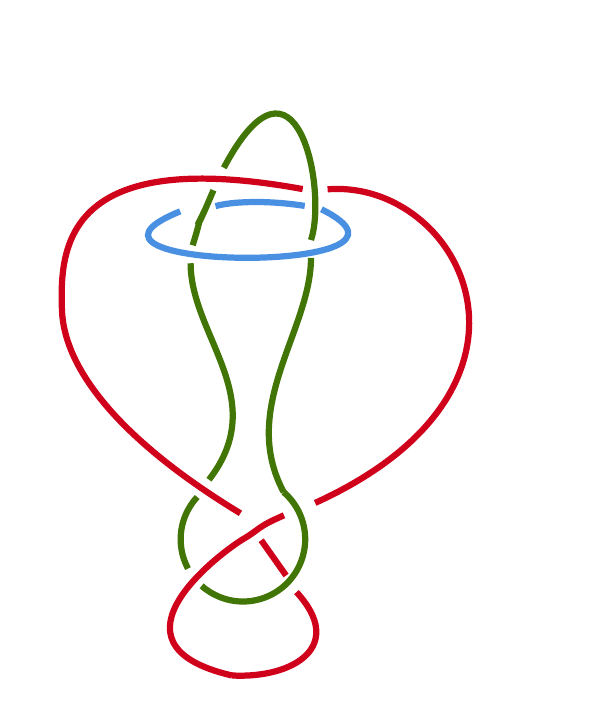
\begin{tikzpicture}[x=0.75pt,y=0.75pt,yscale=-1,xscale=1]
%uncomment if require: \path (0,300); %set diagram left start at 0, and has height of 300

%Curve Lines [id:da09943248726534226] 
\draw [color={rgb, 255:red, 208; green, 2; blue, 27 }  ,draw opacity=1 ][line width=2.25]    (343,46.68) .. controls (407,41.68) and (460,141.77) .. (337,197.77) ;
%Curve Lines [id:da6322873360352863] 
\draw [color={rgb, 255:red, 208; green, 2; blue, 27 }  ,draw opacity=1 ][line width=2.25]    (322,203.75) .. controls (309.03,209.29) and (311.19,209.93) .. (302.21,215.27) .. controls (293.23,220.61) and (231,265.75) .. (297,280.92) ;
%Curve Lines [id:da5011644671112231] 
\draw [color={rgb, 255:red, 208; green, 2; blue, 27 }  ,draw opacity=1 ][line width=2.25]    (331,46.57) .. controls (216,25.57) and (214,74.97) .. (215,104.68) .. controls (216,134.4) and (245,168.77) .. (301,202.77) ;
%Curve Lines [id:da44718777975671287] 
\draw [color={rgb, 255:red, 208; green, 2; blue, 27 }  ,draw opacity=1 ][line width=2.25]    (328,240.75) .. controls (352,266.75) and (326.73,282.41) .. (297,280.92) ;
%Shape: Arc [id:dp40054047053808206] 
\draw  [draw opacity=0][line width=2.25]  (321.85,192.58) .. controls (331.21,200.68) and (334.92,214.11) .. (330.11,226.28) .. controls (324.03,241.69) and (306.61,249.26) .. (291.19,243.17) .. controls (287.84,241.85) and (284.86,239.99) .. (282.31,237.73) -- (302.21,215.27) -- cycle ; \draw  [color={rgb, 255:red, 65; green, 117; blue, 5 }  ,draw opacity=1 ][line width=2.25]  (321.85,192.58) .. controls (331.21,200.68) and (334.92,214.11) .. (330.11,226.28) .. controls (324.03,241.69) and (306.61,249.26) .. (291.19,243.17) .. controls (287.84,241.85) and (284.86,239.99) .. (282.31,237.73) ;  
%Shape: Arc [id:dp11594177788693838] 
\draw  [draw opacity=0][line width=2.25]  (275.74,229.39) .. controls (271.75,221.9) and (270.94,212.77) .. (274.3,204.25) .. controls (275.71,200.7) and (277.71,197.56) .. (280.16,194.91) -- (302.21,215.27) -- cycle ; \draw  [color={rgb, 255:red, 65; green, 117; blue, 5 }  ,draw opacity=1 ][line width=2.25]  (275.74,229.39) .. controls (271.75,221.9) and (270.94,212.77) .. (274.3,204.25) .. controls (275.71,200.7) and (277.71,197.56) .. (280.16,194.91) ;  
%Straight Lines [id:da5976132825673692] 
\draw [color={rgb, 255:red, 208; green, 2; blue, 27 }  ,draw opacity=1 ][fill={rgb, 255:red, 208; green, 2; blue, 27 }  ,fill opacity=1 ][line width=2.25]    (311,215.75) -- (323,232.75) ;
%Curve Lines [id:da5325527173421334] 
\draw [color={rgb, 255:red, 65; green, 117; blue, 5 }  ,draw opacity=1 ][line width=2.25]    (335,79.68) .. controls (335,114.68) and (300,151.68) .. (321.85,192.58) ;
%Curve Lines [id:da2732197209903964] 
\draw [color={rgb, 255:red, 65; green, 117; blue, 5 }  ,draw opacity=1 ][line width=2.25]    (277,82.3) .. controls (277,117.3) and (316,147.68) .. (285.85,186.58) ;
%Curve Lines [id:da21608820690853647] 
\draw [color={rgb, 255:red, 65; green, 117; blue, 5 }  ,draw opacity=1 ][line width=2.25]    (278,73.65) .. controls (286,47.65) and (274,80.12) .. (288,47.12) ;
%Curve Lines [id:da1149451703987957] 
\draw [color={rgb, 255:red, 65; green, 117; blue, 5 }  ,draw opacity=1 ][line width=2.25]    (335,71.12) .. controls (343,47.12) and (328,-29.7) .. (293,36.3) ;
%Curve Lines [id:da6104443808138464] 
\draw [color={rgb, 255:red, 74; green, 144; blue, 226 }  ,draw opacity=1 ][line width=2.25]    (272,57.3) .. controls (200,86.3) and (405,88.3) .. (340,56.3) ;
%Curve Lines [id:da9503680162575591] 
\draw [color={rgb, 255:red, 74; green, 144; blue, 226 }  ,draw opacity=1 ][line width=2.25]    (289,54.8) .. controls (296,52.68) and (313,51.68) .. (332,54.68) ;




\end{tikzpicture}
}\end{figure}}
			\begin{itemize}
				\onslide<5->{\item \textbf{Eigenvalues:} {\tiny $ \mathcolor{OliveGreen}{ \mathbf{-0.471}, 0.0, 0.333, 0.471, 0.666$}}}\\\onslide<7->{{\tiny $ \mathcolor{red}{   \mathbf{-0.333}, 0.0, 0.127, 0.333, 0.872$}}}
				\onslide<8->{\item \small One eigenvalue is negative $\rightarrow$ \textbf{\textcolor{OliveGreen}{Tripartite Entanglement}}}
				 \end{itemize}
		\end{minipage}%
		\begin{minipage}{0.5\textwidth}
			\tiny  
			\onslide<3->{\begin{align*}
				\rho_{abc} &=
				\left[
				\begin{array}{cccccccc}
				0.333 & 0.333 & 0.0 & 0.0 & 0.0 & 0.0 & 0.0 & 0.333 \\ 
				0.333 & 0.333 & 0.0 & 0.0 & 0.0 & 0.0 & 0.0 & 0.333 \\ 
				0.0 & 0.0 & 0.0 & 0.0 & 0.0 & 0.0 & 0.0 & 0.0 \\ 
				0.0 & 0.0 & 0.0 & 0.0 & 0.0 & 0.0 & 0.0 & 0.0 \\ 
				0.0 & 0.0 & 0.0 & 0.0 & 0.0 & 0.0 & 0.0 & 0.0 \\ 
				0.0 & 0.0 & 0.0 & 0.0 & 0.0 & 0.0 & 0.0 & 0.0 \\ 
				0.0 & 0.0 & 0.0 & 0.0 & 0.0 & 0.0 & 0.0 & 0.0 \\ 
				0.333 & 0.333 & 0.0 & 0.0 & 0.0 & 0.0 & 0.0 & 0.333 \\ 
				\end{array}
				\right]}
				\\
				\onslide<4->{\mathcolor{OliveGreen}{\rho^{T_a}_{abc}} &=
				\left[
				\begin{array}{cccccccc}
				0.333 & 0.333 & 0.0 & 0.0 & 0.0 & 0.0 & 0.0 & 0.0 \\ 
				0.333 & 0.333 & 0.0 & 0.0 & 0.0 & 0.0 & 0.0 & 0.0 \\ 
				0.0 & 0.0 & 0.0 & 0.0 & 0.0 & 0.0 & 0.0 & 0.0 \\ 
				0.0 & 0.0 & 0.0 & 0.0 & 0.333 & 0.333 & 0.0 & 0.0 \\ 
				0.0 & 0.0 & 0.0 & 0.333 & 0.0 & 0.0 & 0.0 & 0.0 \\ 
				0.0 & 0.0 & 0.0 & 0.333 & 0.0 & 0.0 & 0.0 & 0.0 \\ 
				0.0 & 0.0 & 0.0 & 0.0 & 0.0 & 0.0 & 0.0 & 0.0 \\ 
				0.0 & 0.0 & 0.0 & 0.0 & 0.0 & 0.0 & 0.0 & 0.333 \\ 
				\end{array}
				\right]}
				\\
				\onslide<6->{\mathcolor{red}{\rho^{T_c}_{abc}} &=
				\left[
				\begin{array}{cccccccc}
				0.333 & 0.333 & 0.0 & 0.0 & 0.0 & 0.0 & 0.0 & 0.0 \\ 
				0.333 & 0.333 & 0.0 & 0.0 & 0.0 & 0.0 & 0.333 & 0.333 \\ 
				0.0 & 0.0 & 0.0 & 0.0 & 0.0 & 0.0 & 0.0 & 0.0 \\ 
				0.0 & 0.0 & 0.0 & 0.0 & 0.0 & 0.0 & 0.0 & 0.0 \\ 
				0.0 & 0.0 & 0.0 & 0.0 & 0.0 & 0.0 & 0.0 & 0.0 \\ 
				0.0 & 0.0 & 0.0 & 0.0 & 0.0 & 0.0 & 0.0 & 0.0 \\ 
				0.0 & 0.333 & 0.0 & 0.0 & 0.0 & 0.0 & 0.0 & 0.0 \\ 
				0.0 & 0.333 & 0.0 & 0.0 & 0.0 & 0.0 & 0.0 & 0.333 \\ 
				\end{array}
				\right]}
				\end{align*}
		\end{minipage}
	\end{frame}

	\begin{frame}{\textbf{Three Qubit System}: 3\textsuperscript{2} class: cut}
		\onslide<1->{\textcolor{red}{\textbf{Pure State:} } $\ket{3^2}_{abc} = \frac{1}{\sqrt{3}}\brac{\ket{000}_{abc} + \ket{111}_{abc} + \ket{001}_{abc}} $\\[0.3cm]}
		\begin{minipage}{0.35\textwidth}
			%

\tikzset{every picture/.style={line width=0.75pt}} %set default line width to 0.75pt        

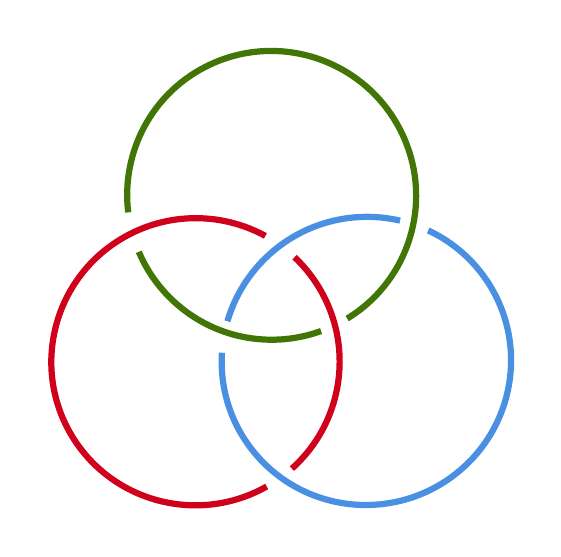
\begin{tikzpicture}[x=0.75pt,y=0.75pt,yscale=-1,xscale=1]
%uncomment if require: \path (0,300); %set diagram left start at 0, and has height of 300

%Shape: Arc [id:dp49278097545949884] 
\draw  [draw opacity=0][line width=2.25]  (328.62,163.73) .. controls (321.19,166.44) and (313.18,167.92) .. (304.82,167.92) .. controls (276.06,167.92) and (251.39,150.46) .. (240.8,125.56) -- (304.82,98.33) -- cycle ; \draw  [color={rgb, 255:red, 65; green, 117; blue, 5 }  ,draw opacity=1 ][line width=2.25]  (328.62,163.73) .. controls (321.19,166.44) and (313.18,167.92) .. (304.82,167.92) .. controls (276.06,167.92) and (251.39,150.46) .. (240.8,125.56) ;  
%Shape: Arc [id:dp7313937278600963] 
\draw  [draw opacity=0][line width=2.25]  (380.22,115.26) .. controls (389.75,119.69) and (398.4,126.36) .. (405.34,135.15) .. controls (429.07,165.23) and (423.73,208.87) .. (393.41,232.62) .. controls (363.09,256.37) and (319.27,251.24) .. (295.54,221.15) .. controls (284.6,207.29) and (279.84,190.54) .. (280.85,174.18) -- (350.44,178.15) -- cycle ; \draw  [color={rgb, 255:red, 74; green, 144; blue, 226 }  ,draw opacity=1 ][line width=2.25]  (380.22,115.26) .. controls (389.75,119.69) and (398.4,126.36) .. (405.34,135.15) .. controls (429.07,165.23) and (423.73,208.87) .. (393.41,232.62) .. controls (363.09,256.37) and (319.27,251.24) .. (295.54,221.15) .. controls (284.6,207.29) and (279.84,190.54) .. (280.85,174.18) ;  
%Shape: Arc [id:dp9082888658781946] 
\draw  [draw opacity=0][line width=2.25]  (235.71,106.58) .. controls (232.15,77.58) and (247.26,48.37) .. (275.16,35.34) .. controls (309.93,19.08) and (351.4,34.11) .. (367.78,68.91) .. controls (383.06,101.37) and (371.11,139.56) .. (341.2,157.73) -- (304.82,98.33) -- cycle ; \draw  [color={rgb, 255:red, 65; green, 117; blue, 5 }  ,draw opacity=1 ][line width=2.25]  (235.71,106.58) .. controls (232.15,77.58) and (247.26,48.37) .. (275.16,35.34) .. controls (309.93,19.08) and (351.4,34.11) .. (367.78,68.91) .. controls (383.06,101.37) and (371.11,139.56) .. (341.2,157.73) ;  
%Shape: Arc [id:dp7357603003827937] 
\draw  [draw opacity=0][line width=2.25]  (302.44,238.64) .. controls (269.08,257.52) and (226.71,245.99) .. (207.75,212.86) .. controls (188.77,179.69) and (200.44,137.44) .. (233.81,118.48) .. controls (255.62,106.09) and (281.32,106.72) .. (301.8,117.92) -- (268.17,178.53) -- cycle ; \draw  [color={rgb, 255:red, 208; green, 2; blue, 27 }  ,draw opacity=1 ][line width=2.25]  (302.44,238.64) .. controls (269.08,257.52) and (226.71,245.99) .. (207.75,212.86) .. controls (188.77,179.69) and (200.44,137.44) .. (233.81,118.48) .. controls (255.62,106.09) and (281.32,106.72) .. (301.8,117.92) ;  
%Shape: Arc [id:dp02993817280793909] 
\draw  [draw opacity=0][line width=2.25]  (283.51,159.01) .. controls (286.66,148.19) and (292.5,137.97) .. (301.03,129.39) .. controls (318.8,111.52) and (343.85,105.22) .. (366.69,110.55) -- (350.44,178.15) -- cycle ; \draw  [color={rgb, 255:red, 74; green, 144; blue, 226 }  ,draw opacity=1 ][line width=2.25]  (283.51,159.01) .. controls (286.66,148.19) and (292.5,137.97) .. (301.03,129.39) .. controls (318.8,111.52) and (343.85,105.22) .. (366.69,110.55) ;  
%Shape: Arc [id:dp6464277844327507] 
\draw  [draw opacity=0][line width=2.25]  (315.85,128.16) .. controls (331.94,143.37) and (340.46,165.99) .. (336.68,189.48) .. controls (334.06,205.76) and (325.96,219.8) .. (314.56,230.03) -- (268.17,178.53) -- cycle ; \draw  [color={rgb, 255:red, 208; green, 2; blue, 27 }  ,draw opacity=1 ][line width=2.25]  (315.85,128.16) .. controls (331.94,143.37) and (340.46,165.99) .. (336.68,189.48) .. controls (334.06,205.76) and (325.96,219.8) .. (314.56,230.03) ;  




\end{tikzpicture}
  % Make sure this file exists
			\begin{figure}
				\onslide<2->{\scalebox{0.4}{

\tikzset{every picture/.style={line width=0.75pt}} %set default line width to 0.75pt        

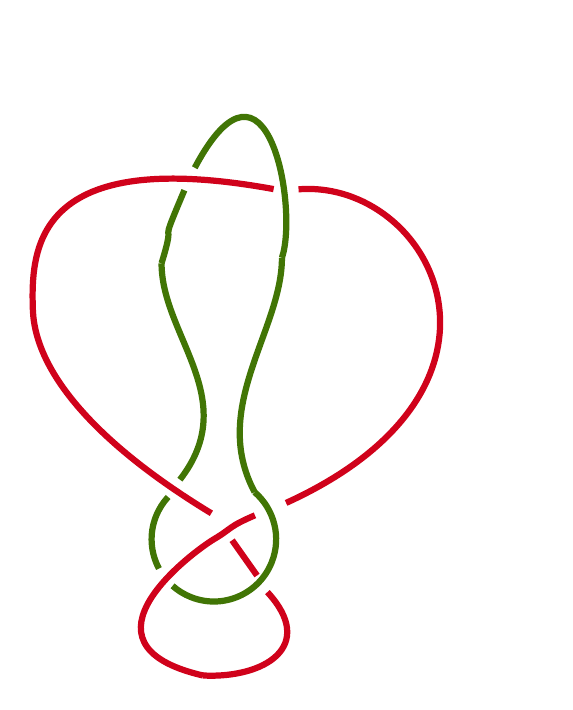
\begin{tikzpicture}[x=0.75pt,y=0.75pt,yscale=-1,xscale=1]
%uncomment if require: \path (0,300); %set diagram left start at 0, and has height of 300

%Curve Lines [id:da7443271823139895] 
\draw [color={rgb, 255:red, 208; green, 2; blue, 27 }  ,draw opacity=1 ][line width=2.25]    (343,46.68) .. controls (407,41.68) and (460,141.77) .. (337,197.77) ;
%Curve Lines [id:da24399078546827557] 
\draw [color={rgb, 255:red, 208; green, 2; blue, 27 }  ,draw opacity=1 ][line width=2.25]    (322,203.75) .. controls (309.03,209.29) and (311.19,209.93) .. (302.21,215.27) .. controls (293.23,220.61) and (231,265.75) .. (297,280.92) ;
%Curve Lines [id:da5476524533721545] 
\draw [color={rgb, 255:red, 208; green, 2; blue, 27 }  ,draw opacity=1 ][line width=2.25]    (331,46.57) .. controls (216,25.57) and (214,74.97) .. (215,104.68) .. controls (216,134.4) and (245,168.77) .. (301,202.77) ;
%Curve Lines [id:da09747722923918067] 
\draw [color={rgb, 255:red, 208; green, 2; blue, 27 }  ,draw opacity=1 ][line width=2.25]    (328,240.75) .. controls (352,266.75) and (326.73,282.41) .. (297,280.92) ;
%Shape: Arc [id:dp7905415087946832] 
\draw  [draw opacity=0][line width=2.25]  (321.85,192.58) .. controls (331.21,200.68) and (334.92,214.11) .. (330.11,226.28) .. controls (324.03,241.69) and (306.61,249.26) .. (291.19,243.17) .. controls (287.84,241.85) and (284.86,239.99) .. (282.31,237.73) -- (302.21,215.27) -- cycle ; \draw  [color={rgb, 255:red, 65; green, 117; blue, 5 }  ,draw opacity=1 ][line width=2.25]  (321.85,192.58) .. controls (331.21,200.68) and (334.92,214.11) .. (330.11,226.28) .. controls (324.03,241.69) and (306.61,249.26) .. (291.19,243.17) .. controls (287.84,241.85) and (284.86,239.99) .. (282.31,237.73) ;  
%Shape: Arc [id:dp9636288395339626] 
\draw  [draw opacity=0][line width=2.25]  (275.74,229.39) .. controls (271.75,221.9) and (270.94,212.77) .. (274.3,204.25) .. controls (275.71,200.7) and (277.71,197.56) .. (280.16,194.91) -- (302.21,215.27) -- cycle ; \draw  [color={rgb, 255:red, 65; green, 117; blue, 5 }  ,draw opacity=1 ][line width=2.25]  (275.74,229.39) .. controls (271.75,221.9) and (270.94,212.77) .. (274.3,204.25) .. controls (275.71,200.7) and (277.71,197.56) .. (280.16,194.91) ;  
%Straight Lines [id:da2186127141902522] 
\draw [color={rgb, 255:red, 208; green, 2; blue, 27 }  ,draw opacity=1 ][fill={rgb, 255:red, 208; green, 2; blue, 27 }  ,fill opacity=1 ][line width=2.25]    (311,215.75) -- (323,232.75) ;
%Curve Lines [id:da09746020631322583] 
\draw [color={rgb, 255:red, 65; green, 117; blue, 5 }  ,draw opacity=1 ][line width=2.25]    (335,79.68) .. controls (335,114.68) and (300,151.68) .. (321.85,192.58) ;
%Curve Lines [id:da25917359230011294] 
\draw [color={rgb, 255:red, 65; green, 117; blue, 5 }  ,draw opacity=1 ][line width=2.25]    (277,82.3) .. controls (277,117.3) and (316,147.68) .. (285.85,186.58) ;
%Curve Lines [id:da698321716307497] 
\draw [color={rgb, 255:red, 65; green, 117; blue, 5 }  ,draw opacity=1 ][line width=2.25]    (277,82.3) .. controls (285,56.3) and (274,80.12) .. (288,47.12) ;
%Curve Lines [id:da17510978624657203] 
\draw [color={rgb, 255:red, 65; green, 117; blue, 5 }  ,draw opacity=1 ][line width=2.25]    (335,79.68) .. controls (343,55.68) and (328,-29.7) .. (293,36.3) ;




\end{tikzpicture}
}}\end{figure}
			\begin{itemize}
				\onslide<5->{\item \textbf{Eigenvalues:} {\footnotesize $\mathcolor{OliveGreen}{0.333,{\mathbf{-0.333}}, 0.666$}}}
				\onslide<6->{\item \small One eigenvalue is negative $\rightarrow$ \textbf{\textcolor{OliveGreen}{Tripartite Entanglement}}}
				 \end{itemize}
		\end{minipage}%
		\begin{minipage}{0.5\textwidth}
		\footnotesize
			\begin{align*}
				\onslide<3->{\rho_{ab} &=
                    \left[
                    \begin{array}{cccc}
                    0.666 & 0.0 & 0.0 & 0.333 \\
                    0.0 & 0.0 & 0.0 & 0.0 \\
                    0.0 & 0.0 & 0.0 & 0.0 \\
                    0.333 & 0.0 & 0.0 & 0.333 \\
                    \end{array}
                    \right]}\\
					\onslide<4->{\mathcolor{OliveGreen}{\rho_{ab}^{T_a}} &=
				 \left[
                    \begin{array}{cccc}
                    0.666 & 0.0 & 0.0 & 0.0 \\
                    0.0 & 0.0 & 0.333 & 0.0 \\
                    0.0 & 0.333 & 0.0 & 0.0 \\
                    0.0 & 0.0 & 0.0 & 0.333 \\
                    \end{array}
                    \right]}\\
				\end{align*}
		\end{minipage}
	\end{frame}




	\begin{frame}{\textbf{Three Qubit System}: 3\textsuperscript{2} class: another cut}
		\onslide<1->{\textcolor{red}{\textbf{Pure State:} } $\ket{3^2}_{abc} = \frac{1}{\sqrt{3}}\brac{\ket{000}_{abc} + \ket{111}_{abc} + \ket{001}_{abc}} $}\\[0.3cm]
		\begin{minipage}{0.35\textwidth}
			%

\tikzset{every picture/.style={line width=0.75pt}} %set default line width to 0.75pt        

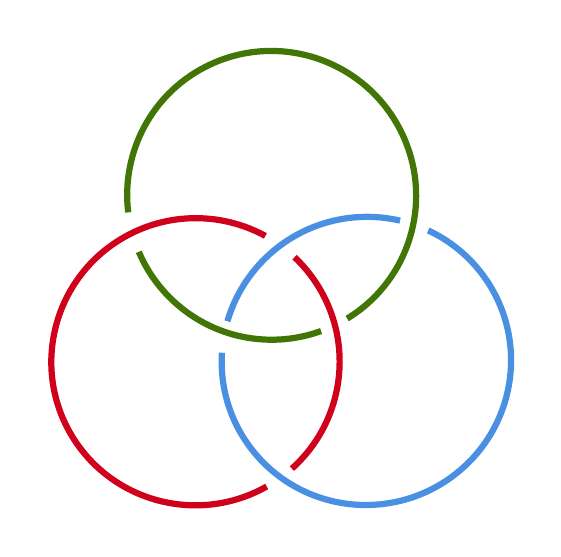
\begin{tikzpicture}[x=0.75pt,y=0.75pt,yscale=-1,xscale=1]
%uncomment if require: \path (0,300); %set diagram left start at 0, and has height of 300

%Shape: Arc [id:dp49278097545949884] 
\draw  [draw opacity=0][line width=2.25]  (328.62,163.73) .. controls (321.19,166.44) and (313.18,167.92) .. (304.82,167.92) .. controls (276.06,167.92) and (251.39,150.46) .. (240.8,125.56) -- (304.82,98.33) -- cycle ; \draw  [color={rgb, 255:red, 65; green, 117; blue, 5 }  ,draw opacity=1 ][line width=2.25]  (328.62,163.73) .. controls (321.19,166.44) and (313.18,167.92) .. (304.82,167.92) .. controls (276.06,167.92) and (251.39,150.46) .. (240.8,125.56) ;  
%Shape: Arc [id:dp7313937278600963] 
\draw  [draw opacity=0][line width=2.25]  (380.22,115.26) .. controls (389.75,119.69) and (398.4,126.36) .. (405.34,135.15) .. controls (429.07,165.23) and (423.73,208.87) .. (393.41,232.62) .. controls (363.09,256.37) and (319.27,251.24) .. (295.54,221.15) .. controls (284.6,207.29) and (279.84,190.54) .. (280.85,174.18) -- (350.44,178.15) -- cycle ; \draw  [color={rgb, 255:red, 74; green, 144; blue, 226 }  ,draw opacity=1 ][line width=2.25]  (380.22,115.26) .. controls (389.75,119.69) and (398.4,126.36) .. (405.34,135.15) .. controls (429.07,165.23) and (423.73,208.87) .. (393.41,232.62) .. controls (363.09,256.37) and (319.27,251.24) .. (295.54,221.15) .. controls (284.6,207.29) and (279.84,190.54) .. (280.85,174.18) ;  
%Shape: Arc [id:dp9082888658781946] 
\draw  [draw opacity=0][line width=2.25]  (235.71,106.58) .. controls (232.15,77.58) and (247.26,48.37) .. (275.16,35.34) .. controls (309.93,19.08) and (351.4,34.11) .. (367.78,68.91) .. controls (383.06,101.37) and (371.11,139.56) .. (341.2,157.73) -- (304.82,98.33) -- cycle ; \draw  [color={rgb, 255:red, 65; green, 117; blue, 5 }  ,draw opacity=1 ][line width=2.25]  (235.71,106.58) .. controls (232.15,77.58) and (247.26,48.37) .. (275.16,35.34) .. controls (309.93,19.08) and (351.4,34.11) .. (367.78,68.91) .. controls (383.06,101.37) and (371.11,139.56) .. (341.2,157.73) ;  
%Shape: Arc [id:dp7357603003827937] 
\draw  [draw opacity=0][line width=2.25]  (302.44,238.64) .. controls (269.08,257.52) and (226.71,245.99) .. (207.75,212.86) .. controls (188.77,179.69) and (200.44,137.44) .. (233.81,118.48) .. controls (255.62,106.09) and (281.32,106.72) .. (301.8,117.92) -- (268.17,178.53) -- cycle ; \draw  [color={rgb, 255:red, 208; green, 2; blue, 27 }  ,draw opacity=1 ][line width=2.25]  (302.44,238.64) .. controls (269.08,257.52) and (226.71,245.99) .. (207.75,212.86) .. controls (188.77,179.69) and (200.44,137.44) .. (233.81,118.48) .. controls (255.62,106.09) and (281.32,106.72) .. (301.8,117.92) ;  
%Shape: Arc [id:dp02993817280793909] 
\draw  [draw opacity=0][line width=2.25]  (283.51,159.01) .. controls (286.66,148.19) and (292.5,137.97) .. (301.03,129.39) .. controls (318.8,111.52) and (343.85,105.22) .. (366.69,110.55) -- (350.44,178.15) -- cycle ; \draw  [color={rgb, 255:red, 74; green, 144; blue, 226 }  ,draw opacity=1 ][line width=2.25]  (283.51,159.01) .. controls (286.66,148.19) and (292.5,137.97) .. (301.03,129.39) .. controls (318.8,111.52) and (343.85,105.22) .. (366.69,110.55) ;  
%Shape: Arc [id:dp6464277844327507] 
\draw  [draw opacity=0][line width=2.25]  (315.85,128.16) .. controls (331.94,143.37) and (340.46,165.99) .. (336.68,189.48) .. controls (334.06,205.76) and (325.96,219.8) .. (314.56,230.03) -- (268.17,178.53) -- cycle ; \draw  [color={rgb, 255:red, 208; green, 2; blue, 27 }  ,draw opacity=1 ][line width=2.25]  (315.85,128.16) .. controls (331.94,143.37) and (340.46,165.99) .. (336.68,189.48) .. controls (334.06,205.76) and (325.96,219.8) .. (314.56,230.03) ;  




\end{tikzpicture}
  % Make sure this file exists
			\begin{figure}
				\onslide<2->{\scalebox{0.4}{

\tikzset{every picture/.style={line width=0.75pt}} %set default line width to 0.75pt        

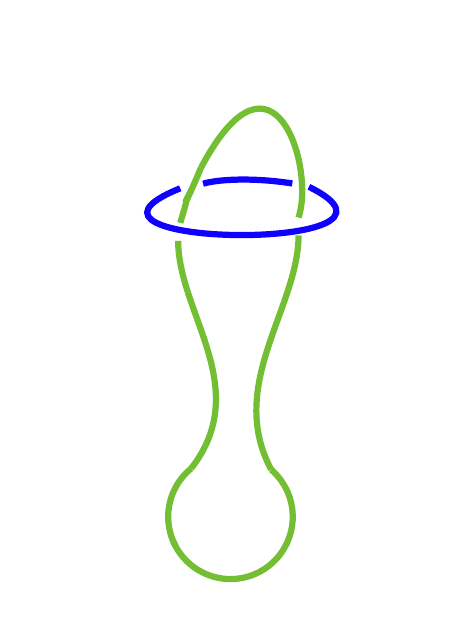
\begin{tikzpicture}[x=0.75pt,y=0.75pt,yscale=-1,xscale=1]
%uncomment if require: \path (0,300); %set diagram left start at 0, and has height of 300

%Shape: Arc [id:dp21168646143636116] 
\draw  [draw opacity=0][line width=2.25]  (321.85,192.58) .. controls (331.21,200.68) and (334.92,214.11) .. (330.11,226.28) .. controls (324.03,241.69) and (306.61,249.26) .. (291.19,243.17) .. controls (283.51,240.14) and (277.78,234.29) .. (274.71,227.27) -- (302.21,215.27) -- cycle ; \draw  [color={rgb, 255:red, 115; green, 190; blue, 50 }  ,draw opacity=1 ][line width=2.25]  (321.85,192.58) .. controls (331.21,200.68) and (334.92,214.11) .. (330.11,226.28) .. controls (324.03,241.69) and (306.61,249.26) .. (291.19,243.17) .. controls (283.51,240.14) and (277.78,234.29) .. (274.71,227.27) ;  
%Shape: Arc [id:dp7304033012343536] 
\draw  [draw opacity=0][line width=2.25]  (275.74,229.39) .. controls (271.75,221.9) and (270.94,212.77) .. (274.3,204.25) .. controls (276.26,199.3) and (279.39,195.15) .. (283.25,192.01) -- (302.21,215.27) -- cycle ; \draw  [color={rgb, 255:red, 115; green, 190; blue, 50 }  ,draw opacity=1 ][line width=2.25]  (275.74,229.39) .. controls (271.75,221.9) and (270.94,212.77) .. (274.3,204.25) .. controls (276.26,199.3) and (279.39,195.15) .. (283.25,192.01) ;  
%Curve Lines [id:da08845374014848362] 
\draw [color={rgb, 255:red, 115; green, 190; blue, 50 }  ,draw opacity=1 ][line width=2.25]    (335,79.68) .. controls (335,114.68) and (300,151.68) .. (321.85,192.58) ;
%Curve Lines [id:da38795962135966966] 
\draw [color={rgb, 255:red, 115; green, 190; blue, 50 }  ,draw opacity=1 ][line width=2.25]    (277,82.3) .. controls (277,117.3) and (313.4,153.11) .. (283.25,192.01) ;
%Curve Lines [id:da55034677237778] 
\draw [color={rgb, 255:red, 115; green, 190; blue, 50 }  ,draw opacity=1 ][line width=2.25]    (278,73.65) .. controls (286,47.65) and (274,80.12) .. (288,47.12) ;
%Curve Lines [id:da8611153062481857] 
\draw [color={rgb, 255:red, 115; green, 190; blue, 50 }  ,draw opacity=1 ][line width=2.25]    (335,71.12) .. controls (343,47.12) and (323,-18.88) .. (288,47.12) ;
%Curve Lines [id:da7227634588793097] 
\draw [color={rgb, 255:red, 15; green, 0; blue, 255 }  ,draw opacity=1 ][line width=2.25]    (278,57.02) .. controls (206,86.02) and (405,88.3) .. (340,56.3) ;
%Curve Lines [id:da6158714712059778] 
\draw [color={rgb, 255:red, 15; green, 0; blue, 255 }  ,draw opacity=1 ][line width=2.25]    (289,54.8) .. controls (296,52.68) and (313,51.68) .. (332,54.68) ;




\end{tikzpicture}
}}\end{figure}
			\begin{itemize}
				\onslide<5->{\item \textbf{Eigenvalues:} {\footnotesize{\footnotesize $\mathcolor{red}{ 0.0, 0.333, 0.666$}}}}
				\onslide<6->{\item \small No eigenvalue is negative $\rightarrow$ \textbf{\textcolor{red}{Separable}}}
				 \end{itemize}
		\end{minipage}%
		\begin{minipage}{0.5\textwidth}
		\footnotesize
			\begin{align*}
				\onslide<3->{\rho_{bc} &=
					\left[
					\begin{array}{cccc}
					0.333 & 0.333 & 0.0 & 0.0 \\
					0.333 & 0.333 & 0.0 & 0.0 \\
					0.0 & 0.0 & 0.0 & 0.0 \\
					0.0 & 0.0 & 0.0 & 0.333 \\
					\end{array}
					\right]}\\
					\onslide<4->{\mathcolor{red}{\rho^{T_b}_{bc}}&=
                \left[
                \begin{array}{cccc}
                0.333 & 0.333 & 0.0 & 0.0 \\
                0.333 & 0.333 & 0.0 & 0.0 \\
                0.0 & 0.0 & 0.0 & 0.0 \\
                0.0 & 0.0 & 0.0 & 0.333 \\
                \end{array}
                \right]}
				\end{align*}
		\end{minipage}
	\end{frame}





	\begin{frame}{\textbf{Four Qubit System}}
		Link Class: $4^{20}$
		
		Link polynomial: $abc+ abd + ac$
		\begin{equation*}
			\ket{\psi_{20}} = \ket{3^1}_{abc}\ket{0}_{d} \ket{0}_e + \ket{3^1}_{abd} \ket{0}_c \ket{1}_e + \ket{2^1}_{ac} \ket{10}_{bd} \ket{2}_e.
		\end{equation*}
		\begin{figure}
			\centering
			\scalebox{0.5}{

\tikzset{every picture/.style={line width=0.75pt}} %set default line width to 0.75pt        

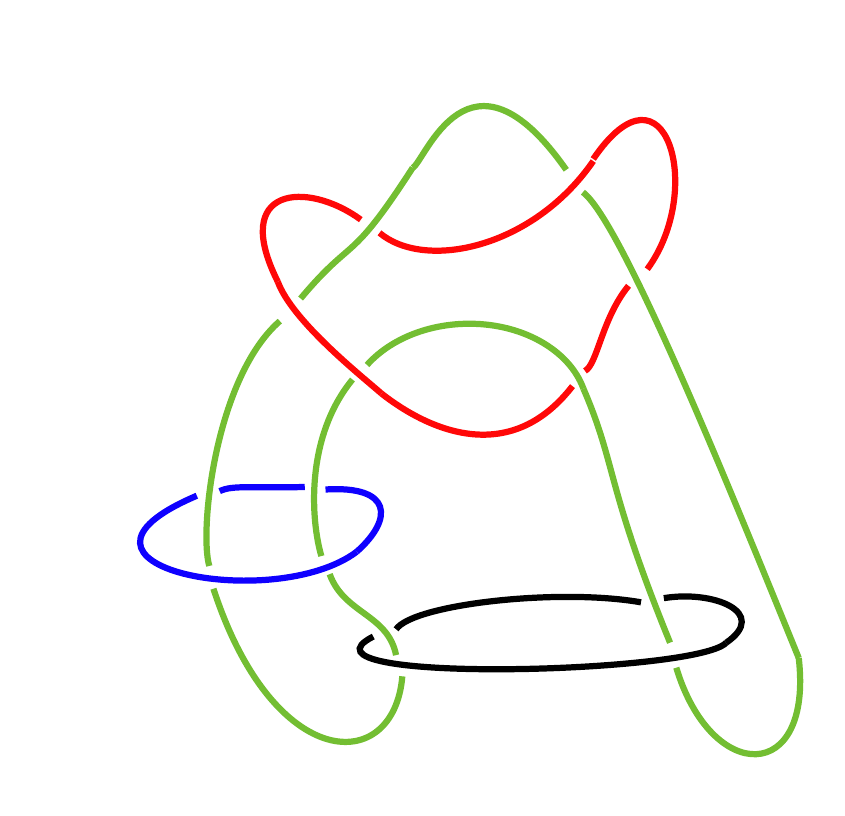
\begin{tikzpicture}[x=0.75pt,y=0.75pt,yscale=-1,xscale=1]
%uncomment if require: \path (0,424); %set diagram left start at 0, and has height of 424

%Curve Lines [id:da7440942804501696] 
\draw [color={rgb, 255:red, 115; green, 190; blue, 50 }  ,draw opacity=1 ][line width=2.25]    (137,283.92) .. controls (132,266.92) and (140,192.93) .. (171,165.93) ;
%Curve Lines [id:da6049310631713473] 
\draw [color={rgb, 255:red, 115; green, 190; blue, 50 }  ,draw opacity=1 ][line width=2.25]    (139,294.88) .. controls (168,383.97) and (226,385.08) .. (230,337.08) ;
%Curve Lines [id:da1349162502759098] 
\draw [color={rgb, 255:red, 15; green, 0; blue, 255 }  ,draw opacity=1 ][line width=2.25]    (131,250.08) .. controls (51,284.08) and (168,307.08) .. (208,277.08) ;
%Curve Lines [id:da11531341974542786] 
\draw [color={rgb, 255:red, 115; green, 190; blue, 50 }  ,draw opacity=1 ][line width=2.25]    (191,279.15) .. controls (186,262.15) and (183,222.08) .. (206,194.08) ;
%Curve Lines [id:da4116440180075853] 
\draw [color={rgb, 255:red, 15; green, 0; blue, 255 }  ,draw opacity=1 ][line width=2.25]    (193,247.08) .. controls (225,245.08) and (226,261.08) .. (208,277.08) ;
%Curve Lines [id:da0486515743629119] 
\draw [color={rgb, 255:red, 15; green, 0; blue, 255 }  ,draw opacity=1 ][line width=2.25]    (142,247.87) .. controls (148,244.87) and (158,246.43) .. (183,245.87) ;
%Curve Lines [id:da11378123258947304] 
\draw [color={rgb, 255:red, 115; green, 190; blue, 50 }  ,draw opacity=1 ][line width=2.25]    (227,326.87) .. controls (223,307.05) and (202,307.05) .. (195,287.87) ;
%Curve Lines [id:da6619932089503573] 
\draw [line width=2.25]    (216,317.92) .. controls (171,340.92) and (372,335.92) .. (386,320.92) ;
%Shape: Arc [id:dp43544062144545004] 
\draw  [draw opacity=0][line width=2.25]  (213,187.08) .. controls (223.16,175.68) and (240.2,167.89) .. (259.73,167.25) .. controls (287.04,166.35) and (310.41,179.69) .. (317.25,198.48) -- (261.17,210.71) -- cycle ; \draw  [color={rgb, 255:red, 115; green, 190; blue, 50 }  ,draw opacity=1 ][line width=2.25]  (213,187.08) .. controls (223.16,175.68) and (240.2,167.89) .. (259.73,167.25) .. controls (287.04,166.35) and (310.41,179.69) .. (317.25,198.48) ;  
%Curve Lines [id:da37840307283624053] 
\draw [color={rgb, 255:red, 115; green, 190; blue, 50 }  ,draw opacity=1 ][line width=2.25]    (317.25,198.48) .. controls (333.25,235.48) and (328,244.87) .. (359,320.87) ;
%Curve Lines [id:da9236552868680381] 
\draw [color={rgb, 255:red, 115; green, 190; blue, 50 }  ,draw opacity=1 ][line width=2.25]    (362,332.92) .. controls (379,389.27) and (428,389.27) .. (421,328.27) ;
%Curve Lines [id:da1086285435159654] 
\draw [color={rgb, 255:red, 115; green, 190; blue, 50 }  ,draw opacity=1 ][line width=2.25]    (317,103.85) .. controls (336,118.02) and (390,252.27) .. (421,328.27) ;
%Curve Lines [id:da7567172706629643] 
\draw [line width=2.25]    (356,299.43) .. controls (380,295.43) and (407,306.43) .. (386,320.92) ;
%Curve Lines [id:da5766459881001758] 
\draw [line width=2.25]    (227,314.43) .. controls (235,302.43) and (305,294.43) .. (345,301.43) ;
%Curve Lines [id:da5195577821405296] 
\draw [color={rgb, 255:red, 255; green, 8; blue, 8 }  ,draw opacity=1 ][line width=2.25]    (220,200.87) .. controls (211,192.93) and (177,166.12) .. (170,146.93) ;
%Curve Lines [id:da4987177132002978] 
\draw [color={rgb, 255:red, 255; green, 8; blue, 8 }  ,draw opacity=1 ][line width=2.25]    (170,146.93) .. controls (147,101.07) and (184,98.07) .. (210,117.07) ;
%Curve Lines [id:da9817882212140966] 
\draw [color={rgb, 255:red, 115; green, 190; blue, 50 }  ,draw opacity=1 ][line width=2.25]    (181,155.07) .. controls (207,124.07) and (204,140.07) .. (235,92.07) ;
%Curve Lines [id:da032233278465274684] 
\draw [color={rgb, 255:red, 115; green, 190; blue, 50 }  ,draw opacity=1 ][line width=2.25]    (235,92.07) .. controls (241,89.07) and (262,26.07) .. (309,93.07) ;
%Curve Lines [id:da19253558134933546] 
\draw [color={rgb, 255:red, 255; green, 8; blue, 8 }  ,draw opacity=1 ][line width=2.25]    (219,123.43) .. controls (241,141.85) and (293,130.85) .. (322,88.85) ;
%Curve Lines [id:da47798653538396874] 
\draw [color={rgb, 255:red, 255; green, 8; blue, 8 }  ,draw opacity=1 ][line width=2.25]    (322,87.85) .. controls (357,36.33) and (376,102.93) .. (348,140.93) ;
%Curve Lines [id:da9480456662349792] 
\draw [color={rgb, 255:red, 255; green, 8; blue, 8 }  ,draw opacity=1 ][line width=2.25]    (220,200.87) .. controls (241,217.33) and (281,237.27) .. (312,197.27) ;
%Curve Lines [id:da8609600890787912] 
\draw [color={rgb, 255:red, 255; green, 8; blue, 8 }  ,draw opacity=1 ][line width=2.25]    (318,189.93) .. controls (324,186.93) and (326,164.82) .. (339,148.93) ;




\end{tikzpicture}
}
		\end{figure}
		a: green    b: black   c: red   d: blue   
		\end{frame}
		
		\begin{frame}{\textbf{Four Qubit System}}
		\begin{equation*}
			\hat{\rho}_{abcd} = \frac{\Tr_e(\ket{\psi_{20}} \bra{\psi_{20}})}{\sqrt{\bra{\psi_{20}} \ket{\psi_{20}}}}.
		\end{equation*}
		We need to check for Four-partite entanglement. So we have to compute the eigenvalues of the partial transpose with respect to each subsystem.
		\begin{equation*}
		\begin{split}
			&\hat{\rho}^{T_a}_{abcd} : \text{ Eigenvalues: } -0.270, -0.103, 0.000, 0.103, 0.270, 0.333 \\
			&\hat{\rho}^{T_b}_{abcd}: \text{ Eigenvalues: } -0.186, 0.000, 0.167, 0.209, 0.333, 0.477 \\
			&\hat{\rho}^{T_c}_{abcd}: \text{ Eigenvalues: } -0.236, 0.000, 0.064, 0.167, 0.236, 0.333, 0.436 \\
			&\hat{\rho}^{T_d}_{abcd}: \text{ Eigenvalues: } -0.167, 0.000, 0.033, 0.167, 0.259, 0.541
		\end{split}
		\end{equation*}
		\onslide<2->
		{As the eigenvalues are negative, it has \textbf{FOUR PARTITE ENTANGLEMENT}.}
		\end{frame}
		
		\begin{frame}{\textbf{Four Qubit System}}
		All Possible Partial Traces:
		
		\textbf{Partial Trace with respect to system $a$ :}
		\begin{equation*}
			\hat{\rho}_{bcd} = \left[\begin{matrix}0.333 & 0 & 0 & 0 & 0 & 0 & 0 & 0\\0 & 0 & 0 & 0 & 0 & 0 & 0 & 0\\0 & 0 & 0 & 0 & 0 & 0 & 0 & 0\\0 & 0 & 0 & 0 & 0 & 0 & 0 & 0\\0 & 0 & 0 & 0 & 0.166 & 0 & 0 & 0\\0 & 0 & 0 & 0 & 0 & 0.166 & 0 & 0\\0 & 0 & 0 & 0 & 0 & 0 & 0.333 & 0\\0 & 0 & 0 & 0 & 0 & 0 & 0 & 0\end{matrix}\right].
		\end{equation*}
		As this is a diagonal matrix, we can say directly that after measuring $a$, the rest of the system $b$,$c$,$d$ becomes \textbf{separable}.
		\end{frame}
		
		\begin{frame}{\textbf{Four Qubit System}}
		\textbf{Partial Trace with respect to system $b$ :}
		\begin{itemize}
			\item \onslide<2->$\hat{\rho}_{acd}^{T_a}$:
			\begin{equation*}
				\text{Eigenvalues: }-0.167, 0.000, 0.167, 0.167, 0.333, 0.500.
			\end{equation*}
			\item \onslide<3->$\hat{\rho}_{acd}^{T_c}$:
			\begin{equation*}
				\text{Eigenvalues: }-0.167, 0.000, 0.167, 0.167, 0.333, 0.500.
			\end{equation*}
			\item \onslide<4->$\hat{\rho}_{acd}^{T_d}$:
			\begin{equation*}
				\text{Eigenvalues: }0.000, 0.000, 0.000, 0.167, 0.230, 0.603.
			\end{equation*}
		\end{itemize}
		\onslide<5->{Negative eigenvalues suggest, \textbf{$a$ and $cd$ are entangled}, and \textbf{$c$ and $ad$ are entangled.}}
		\onslide<6->{
		We can not say anything about the subsystem $d$ and $ac$.}
		\end{frame}
		
		\begin{frame}{\textbf{Four Qubit System}}
			\textbf{Partial Trace with respect to system $b$ :}
			
			$\mathcal{Q}.$ How to conclude anything about the separability of the subsystem $d$ and $ac$?
			
			\onslide<2->{
			Computing eigenstates of $\rho_{acd}$:
			
			\begin{equation*}
				\left[\begin{matrix}0\\0\\1.0\\0\\0\\0\\0\\0\end{matrix}\right],
				\left[\begin{matrix}0\\0\\0\\1.0\\0\\0\\0\\0\end{matrix}\right],
				\left[\begin{matrix}0\\0\\0\\0\\1.0\\0\\0\\0\end{matrix}\right],
				\left[\begin{matrix}0\\-1.0\\0\\0\\0\\0\\0\\0\end{matrix}\right],
				\left[\begin{matrix}0\\0\\0\\0\\0\\0\\0\\1.0\end{matrix}\right],
				\left[\begin{matrix}0\\0\\0\\0\\0\\1.0\\0\\0\end{matrix}\right],
				\left[\begin{matrix}0.525\\0\\0\\0\\0\\0\\-0.850\\0\end{matrix}\right],
				\left[\begin{matrix}0.850\\0\\0\\0\\0\\0\\0.525\\0\end{matrix}\right]
			\end{equation*}}
		\onslide<3->{
		If we can show that these vectors are separable as $\ket{v_{ac}} \otimes \ket{v_d}$, then that will show that the $ac$ and $d$ are separable}.
		\end{frame}
		
		\begin{frame}{\textbf{Four Qubit System}}
			\textbf{Partial Trace with respect to system $b$ :}
			
			Consider, 
			\begin{equation*}
				\left[\begin{matrix}0\\0\\1.0\\0\\0\\0\\0\\0\end{matrix}\right] = \ket{0}_a\ket{0}_c\ket{0}_d.
			\end{equation*}
		So this vector is separable in this form $\ket{v_{ac}} \otimes \ket{v_d}$.
		
		Similarly, we can say all the vectors of this form are separable.
		\end{frame}
		
		\begin{frame}{\textbf{Four Qubit System}}
			\textbf{Partial Trace with respect to system $b$ :}
			
			Consider,
			\begin{equation*}
				\left[\begin{matrix}0.525\\0\\0\\0\\0\\0\\-0.850\\0\end{matrix}\right] = 0.525 \ket{0}_a \otimes \ket{0}_c \otimes \ket{0}_d - 0.850 \ket{1}_a \otimes \ket{1}_c \otimes \ket{0}_d
			\end{equation*}
		This can be written as,
		\begin{equation*}
			\begin{split}
			&(0.525\ket{0}_a\otimes \ket{0}_c - 0.850\ket{1}_a\otimes \ket{1}_c) \otimes \ket{0}_d.\\
			=&\ket{v_{ac}} \otimes \ket{v}_d
		\end{split}
		\end{equation*}
		
		\onslide<1->{\textbf{So, $ac$ and $d$ are separable.}}
		\end{frame}
		
		\begin{frame}{\textbf{Four Qubit System}}
			\textbf{Partial Trace with respect to system $c$ :}
			\begin{itemize}
				\item \onslide<2->$\hat{\rho}_{abd}^{T_a}$:
				\begin{equation*}
					\text{Eigenvalues: }-0.167, 0.000, 0.167, 0.167, 0.167, 0.333.
				\end{equation*}
				\item \onslide<3->$\hat{\rho}_{abd}^{T_b}$:
				\begin{equation*}
					\text{Eigenvalues: }-0.103, 0.000, 0.167, 0.270, 0.333, 0.333.
				\end{equation*}
				\item \onslide<4->$\hat{\rho}_{abd}^{T_d}$:
				\begin{equation*}
					\text{Eigenvalues: }-0.069, 0.000,  0.167, 0.167, 0.333, 0.402.
				\end{equation*}
			\end{itemize}
			\onslide<5->{Negative eigenvalues suggest, \textbf{$a$ and $bd$ are entangled}, \textbf{$b$ and $ad$ are entangled.} and \textbf{$d$ and $ab$ are entangled}}.
		\end{frame}
		
		\begin{frame}{\textbf{Four Qubit System}}
			\textbf{Partial Trace with respect to system $d$ :}
			\begin{itemize}
				\item \onslide<2->$\hat{\rho}_{abc}^{T_a}$:
				\begin{equation*}
					\text{Eigenvalues: }-0.208, 0.000, 0.074, 0.167, 0.300, 0.333,
				\end{equation*}
				\item \onslide<3->$\hat{\rho}_{abc}^{T_b}$:
				\begin{equation*}
					\text{Eigenvalues: }-0.122, 0.000, 0.167, 0.167, 0.333, 0.455.
				\end{equation*}
				\item \onslide<4->$\hat{\rho}_{abc}^{T_c}$:
				\begin{equation*}
					\text{Eigenvalues: }-0.167, 0.000, 0.167, 0.333, 0.333, 0.333.
				\end{equation*}
			\end{itemize}
			\onslide<5->{Negative eigenvalues suggest, \textbf{$a$ and $bc$ are entangled}, \textbf{$b$ and $ac$ are entangled.} and \textbf{$c$ and $ab$ are entangled}}.
		\end{frame}
		
		\begin{frame}{\textbf{Four Qubit System}}
			\textbf{Partial Trace with respect to system $ab$ :}
			\begin{equation*}
				\hat{\rho}_{cd} = \left[\begin{matrix}0.5 & 0 & 0 & 0\\0 & 0.166 & 0 & 0\\0 & 0 & 0.333 & 0\\0 & 0 & 0 & 0\end{matrix}\right]
				.
			\end{equation*}
		So, \textbf{$c$ and $d$ are separated.}
		\end{frame}
		
		\begin{frame}{\textbf{Four Qubit System}}
			\textbf{Partial Trace with respect to system $bc$ :}
			\begin{equation*}
				\hat{\rho}_{ad} =\left[\begin{matrix}0.5 & 0 & 0 & 0\\0 & 0 & 0 & 0\\0 & 0 & 0.333 & 0\\0 & 0 & 0 & 0.166\end{matrix}\right]
				.
			\end{equation*}
		So, \textbf{$a$ and $d$ are separated.}
		\end{frame}
		
		\begin{frame}{\textbf{Four Qubit System}}
			\textbf{Partial Trace with respect to system $cd$ :}
			\begin{equation*}
				\hat{\rho}_{ab} = \left[\begin{matrix}0.333 & 0 & 0 & 0\\0 & 0.166 & 0 & 0\\0 & 0 & 0 & 0\\0 & 0 & 0 & 0.5\end{matrix}\right]
				.
			\end{equation*}
		So, \textbf{$a$ and $b$ are separated.}
		\end{frame}
		\begin{frame}{\textbf{Four Qubit System}}
			\textbf{Partial Trace with respect to system $ad$ :}
			\begin{equation*}
				\hat{\rho}_{bc} = \left[\begin{matrix}0.333 & 0 & 0 & 0\\0 & 0 & 0 & 0\\0 & 0 & 0.333 & 0\\0 & 0 & 0 & 0.333\end{matrix}\right]
				.
			\end{equation*}
		So, \textbf{$b$ and $c$ are separated.}
		\end{frame}
		\begin{frame}{\textbf{Four Qubit System}}
			\textbf{Partial Trace with respect to system $bd$ :}
			
			\begin{equation*}
				\hat{\rho}_{ac} = \left[\begin{matrix}0.5 & 0 & 0 & 0.166\\0 & 0 & 0 & 0\\0 & 0 & 0.166 & 0\\0.166 & 0 & 0 & 0.333\end{matrix}\right]
				.
			\end{equation*}
		\end{frame}
		
		\begin{frame}{\textbf{Four Qubit System}}
			Partial Transpose with respect to $a$:
			\begin{equation*}
				\hat{\rho}_{ac}^{T_a} = \left[\begin{matrix}0.5 & 0 & 0 & 0\\0 & 0 & 0.166 & 0\\0 & 0.166 & 0.166 & 0\\0 & 0 & 0 & 0.333\end{matrix}\right].
			\end{equation*}
		Eigenvalues are : -0.103, 0.270, 0.333, 0.500.
		
		So, \textbf{$a$ and $c$ are entangled}.
		\end{frame}
		
		\begin{frame}{\textbf{Four Qubit System}}
			\textbf{Partial Trace with respect to system $ac$ :}
			\begin{equation*}
				\hat{\rho}_{bd} = \left[\begin{matrix}0.333 & 0 & 0 & 0\\0 & 0 & 0 & 0\\0 & 0 & 0.5 & 0\\0 & 0 & 0 & 0.166\end{matrix}\right]
				.
			\end{equation*}
		So, \textbf{$b$ and $d$ are separated.}
		\end{frame}
		
		\begin{frame}{\textbf{Four Qubit System}}
			\textbf{Result:}
			\begin{itemize}
				\item After tracing out $a$, rest of the system $b$, $c$, $d$ becomes separable.
				\item After tracing out $b$, $a$ and $cd$ remain entangled, $c$ and $ad$ remain entangled, and $ac$ and $d$ are separable.
				\item After tracing out $c$, $a$ and $bd$, $b$ and $ad$, and $d$ and $ab$ remain entangled.
				\item After tracing out $d$, $a$ and $bc$, $b$ and $ac$, and $c$ and $ab$ remain entangled.
				\item After tracing out $ab$, $c$ and $d$ are separable.
				\item After tracing out $bc$, $a$ and $d$ are separable.
				\item After tracing out $cd$, $a$ and $d$ are separable.
				\item After tracing out $ad$, $b$ and $c$ are separable.
				\item After tracing out $bd$, $a$ and $c$ are entangled.
				\item After tracing out $ac$, $b$ and $d$ are separable.
			\end{itemize}
		So, \textbf{the polynomial is $abc + abd + ac$.}
		\end{frame}
	\begin{frame}{\textbf{Application to Qubit Networks}}
		\begin{itemize}
			\item \onslide<1-> {Different parties possessing entangled qubits, want to perform protocols with certain restrictions. }
			\item \onslide<3->{If density operator of the subsystem consisting the parties wanting to perform the protocol is separable, then the protocol cannot be performed successfully.}
			\item \onslide<4-> {If another party (not participating in the protocol) does not divulge information about their local operations, then results of the protocol cannot be correlated.}
		\end{itemize}
		\begin{figure}
			\centering
		\onslide<2->{\scalebox{0.6}{

			\tikzset{every picture/.style={line width=0.75pt}} %set default line width to 0.75pt        
			
			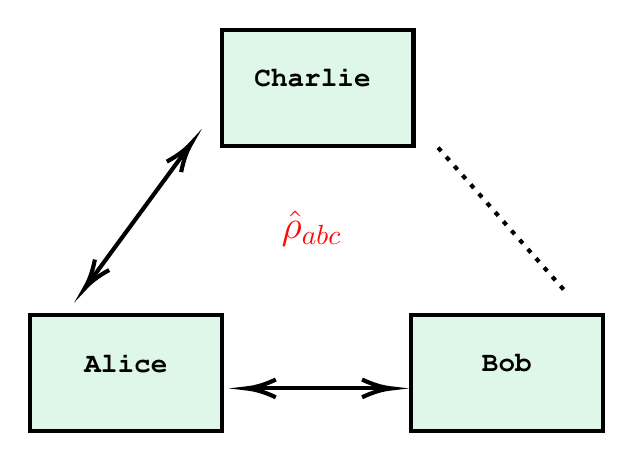
\begin{tikzpicture}[x=0.75pt,y=0.75pt,yscale=-1,xscale=1]
			%uncomment if require: \path (0,300); %set diagram left start at 0, and has height of 300
			
			%Shape: Rectangle [id:dp5199805559721411] 
			\draw  [fill={rgb, 255:red, 223; green, 247; blue, 233 }  ,fill opacity=1 ][line width=1.5]  (197,162.92) -- (289.44,162.92) -- (289.44,218.97) -- (197,218.97) -- cycle ;
			%Shape: Rectangle [id:dp4541164641811364] 
			\draw  [color={rgb, 255:red, 0; green, 0; blue, 0 }  ,draw opacity=1 ][fill={rgb, 255:red, 223; green, 247; blue, 233 }  ,fill opacity=1 ][line width=1.5]  (289.44,25.57) -- (381.88,25.57) -- (381.88,81.63) -- (289.44,81.63) -- cycle ;
			%Shape: Rectangle [id:dp04458970673752716] 
			\draw  [fill={rgb, 255:red, 223; green, 247; blue, 233 }  ,fill opacity=1 ][line width=1.5]  (380.56,162.92) -- (473,162.92) -- (473,218.97) -- (380.56,218.97) -- cycle ;
			%Straight Lines [id:da5905977694939716] 
			\draw [line width=1.5]    (225.19,147.84) -- (273.14,82.6) ;
			\draw [shift={(274.91,80.18)}, rotate = 126.32] [color={rgb, 255:red, 0; green, 0; blue, 0 }  ][line width=1.5]    (14.21,-4.28) .. controls (9.04,-1.82) and (4.3,-0.39) .. (0,0) .. controls (4.3,0.39) and (9.04,1.82) .. (14.21,4.28)   ;
			\draw [shift={(223.41,150.26)}, rotate = 306.32] [color={rgb, 255:red, 0; green, 0; blue, 0 }  ][line width=1.5]    (14.21,-4.28) .. controls (9.04,-1.82) and (4.3,-0.39) .. (0,0) .. controls (4.3,0.39) and (9.04,1.82) .. (14.21,4.28)   ;
			%Straight Lines [id:da10833960790906139] 
			\draw [line width=1.5]  [dash pattern={on 1.69pt off 2.76pt}]  (393.73,82.36) -- (454.47,151.03) ;
			%Straight Lines [id:da635570582048944] 
			\draw [line width=1.5]    (304.33,198.37) -- (368.32,198.37) ;
			\draw [shift={(371.32,198.37)}, rotate = 180] [color={rgb, 255:red, 0; green, 0; blue, 0 }  ][line width=1.5]    (14.21,-4.28) .. controls (9.04,-1.82) and (4.3,-0.39) .. (0,0) .. controls (4.3,0.39) and (9.04,1.82) .. (14.21,4.28)   ;
			\draw [shift={(301.33,198.37)}, rotate = 0] [color={rgb, 255:red, 0; green, 0; blue, 0 }  ][line width=1.5]    (14.21,-4.28) .. controls (9.04,-1.82) and (4.3,-0.39) .. (0,0) .. controls (4.3,0.39) and (9.04,1.82) .. (14.21,4.28)   ;
			
			% Text Node
			\draw (222.06,180.54) node [anchor=north west][inner sep=0.75pt]   [align=left] {{\fontfamily{pcr}\selectfont \textbf{Alice}}};
			% Text Node
			\draw (303.98,43) node [anchor=north west][inner sep=0.75pt]   [align=left] {\textbf{{\fontfamily{pcr}\selectfont Charlie}}};
			% Text Node
			\draw (413.58,180.34) node [anchor=north west][inner sep=0.75pt]   [align=left] {\textbf{{\fontfamily{pcr}\selectfont Bob}}};
			% Text Node
			\draw (317.14,111.48) node [anchor=north west][inner sep=0.75pt]  [font=\Large,color={rgb, 255:red, 255; green, 8; blue, 8 }  ,opacity=1 ]  {$\mathlarger{\mathlarger{{\hat{\rho }_{abc}}}}$};
			
			
			\end{tikzpicture}
			}}
		\end{figure}
	\end{frame}
	\begin{frame}{\textbf{Application to Qubit Networks}}
		Let us consider a four qubit
		network, where Alice, Bob, Charlie and Diana are the parties such that only the following
		parties can communicate:
		\begin{itemize}
			\item \onslide<2->{Alice, Bob, and Charlie}
			\item \onslide<3->{Alice, Bob, and Diana}
			\item \onslide<4->{Alice and Charlie}
		\end{itemize}
		\begin{figure}
			\centering
		\onslide<5->{	\scalebox{0.6}{

		\tikzset{every picture/.style={line width=0.75pt}} %set default line width to 0.75pt        
		
		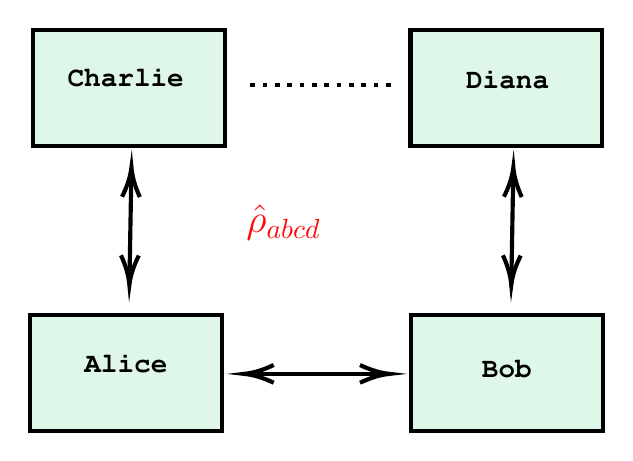
\begin{tikzpicture}[x=0.75pt,y=0.75pt,yscale=-1,xscale=1]
		%uncomment if require: \path (0,300); %set diagram left start at 0, and has height of 300
		
		%Shape: Rectangle [id:dp10277356992512154] 
		\draw  [fill={rgb, 255:red, 223; green, 247; blue, 233 }  ,fill opacity=1 ][line width=1.5]  (197,162.92) -- (289.44,162.92) -- (289.44,218.97) -- (197,218.97) -- cycle ;
		%Shape: Rectangle [id:dp015384298355835657] 
		\draw  [color={rgb, 255:red, 0; green, 0; blue, 0 }  ,draw opacity=1 ][fill={rgb, 255:red, 223; green, 247; blue, 233 }  ,fill opacity=1 ][line width=1.5]  (198.44,25.57) -- (290.88,25.57) -- (290.88,81.63) -- (198.44,81.63) -- cycle ;
		%Shape: Rectangle [id:dp7204404417404228] 
		\draw  [fill={rgb, 255:red, 223; green, 247; blue, 233 }  ,fill opacity=1 ][line width=1.5]  (380.56,162.92) -- (473,162.92) -- (473,218.97) -- (380.56,218.97) -- cycle ;
		%Shape: Rectangle [id:dp17140074186825027] 
		\draw  [color={rgb, 255:red, 0; green, 0; blue, 0 }  ,draw opacity=1 ][fill={rgb, 255:red, 223; green, 247; blue, 233 }  ,fill opacity=1 ][line width=1.5]  (380.44,25.57) -- (472.88,25.57) -- (472.88,81.63) -- (380.44,81.63) -- cycle ;
		%Straight Lines [id:da032463145441033014] 
		\draw [line width=1.5]    (303.33,191.37) -- (367.32,191.37) ;
		\draw [shift={(370.32,191.37)}, rotate = 180] [color={rgb, 255:red, 0; green, 0; blue, 0 }  ][line width=1.5]    (14.21,-4.28) .. controls (9.04,-1.82) and (4.3,-0.39) .. (0,0) .. controls (4.3,0.39) and (9.04,1.82) .. (14.21,4.28)   ;
		\draw [shift={(300.33,191.37)}, rotate = 0] [color={rgb, 255:red, 0; green, 0; blue, 0 }  ][line width=1.5]    (14.21,-4.28) .. controls (9.04,-1.82) and (4.3,-0.39) .. (0,0) .. controls (4.3,0.39) and (9.04,1.82) .. (14.21,4.28)   ;
		%Straight Lines [id:da7055775840806392] 
		\draw [line width=1.5]    (245.05,145.52) -- (245.95,94.88) ;
		\draw [shift={(246,91.88)}, rotate = 91.01] [color={rgb, 255:red, 0; green, 0; blue, 0 }  ][line width=1.5]    (14.21,-4.28) .. controls (9.04,-1.82) and (4.3,-0.39) .. (0,0) .. controls (4.3,0.39) and (9.04,1.82) .. (14.21,4.28)   ;
		\draw [shift={(245,148.52)}, rotate = 271.01] [color={rgb, 255:red, 0; green, 0; blue, 0 }  ][line width=1.5]    (14.21,-4.28) .. controls (9.04,-1.82) and (4.3,-0.39) .. (0,0) .. controls (4.3,0.39) and (9.04,1.82) .. (14.21,4.28)   ;
		%Straight Lines [id:da39607289649694266] 
		\draw [color={rgb, 255:red, 0; green, 0; blue, 0 }  ,draw opacity=1 ][fill={rgb, 255:red, 44; green, 28; blue, 255 }  ,fill opacity=1 ][line width=1.5]    (429.05,145.52) -- (429.95,94.88) ;
		\draw [shift={(430,91.88)}, rotate = 91.01] [color={rgb, 255:red, 0; green, 0; blue, 0 }  ,draw opacity=1 ][line width=1.5]    (14.21,-4.28) .. controls (9.04,-1.82) and (4.3,-0.39) .. (0,0) .. controls (4.3,0.39) and (9.04,1.82) .. (14.21,4.28)   ;
		\draw [shift={(429,148.52)}, rotate = 271.01] [color={rgb, 255:red, 0; green, 0; blue, 0 }  ,draw opacity=1 ][line width=1.5]    (14.21,-4.28) .. controls (9.04,-1.82) and (4.3,-0.39) .. (0,0) .. controls (4.3,0.39) and (9.04,1.82) .. (14.21,4.28)   ;
		%Straight Lines [id:da6546093054475423] 
		\draw [line width=1.5]  [dash pattern={on 1.69pt off 2.76pt}]  (303.33,52.37) -- (332,52.37) -- (373.32,52.37) ;
		
		% Text Node
		\draw (222.06,180.54) node [anchor=north west][inner sep=0.75pt]   [align=left] {{\fontfamily{pcr}\selectfont \textbf{Alice}}};
		% Text Node
		\draw (213.98,43) node [anchor=north west][inner sep=0.75pt]   [align=left] {\textbf{{\fontfamily{pcr}\selectfont Charlie}}};
		% Text Node
		\draw (413.58,183.34) node [anchor=north west][inner sep=0.75pt]   [align=left] {\textbf{{\fontfamily{pcr}\selectfont Bob}}};
		% Text Node
		\draw (300.14,108.48) node [anchor=north west][inner sep=0.75pt]  [font=\Large,color={rgb, 255:red, 255; green, 8; blue, 8 }  ,opacity=1 ]  {$\mathlarger{\mathlarger{\mathlarger{\mathlarger{{\hat{\rho }_{abcd}}}}}}$};
		% Text Node
		\draw (405.98,44) node [anchor=north west][inner sep=0.75pt]   [align=left] {\textbf{{\fontfamily{pcr}\selectfont Diana}}};
		
		
		\end{tikzpicture}
		}}
	
		\end{figure}
		\noindent
		\onslide<6->We can easily see that the polynomial describing this network is $\mathrm{P(a, b, c, d) = abc + abd + ac} \longrightarrow $ \onslide<7->{a state can immediately be constructed from the algorithm}.
	\end{frame}
	\begin{frame}{\textbf{Conclusion}}
		\begin{itemize}
			\onslide<1->{\item We saw how preceding works have tried to use topological links to model entanglement and the problems with such analogies.}
			\onslide<2->{\item We saw how the polynomial approach to entanglement could potentially reduce the ambiguities reflected in the previous works.}
			\onslide<3->{\item We demonstrated a way to obtain a link polynomial from a given entangled state (using the PPT test to check for separability) and also find an entangled state (although mixed) from a given link polynomial.}
			\onslide<4->{\item We then saw some examples demonstrating the procedures for obtaining the links and the states.}
			\onslide<5->{\item We also observed some potential use cases of such an analogy between entanglement and links in qubit networks.}
		\end{itemize}
	
		\onslide<6->{
		\begin{center}
		\begin{minipage}{0.6\textwidth}
			\centering
			
\includegraphics[scale=0.4]{pics/get_calm.png}
		\end{minipage}%
		\hfill
		\begin{minipage}{0.4\textwidth}
			\raggedright
			{\fontsize{24}{28}\selectfont\calligra \textbf{\textcolor{red}{Thank you!}}}
		\end{minipage}
		\end{center}
		}
	\end{frame}
	
\end{document}